\documentclass[10pt,a4paper,twoside]{article}
\RequirePackage{graphicx}
\RequirePackage[british]{babel}
\RequirePackage{bm}
\RequirePackage{courier}
\RequirePackage{microtype}
\RequirePackage[sc]{mathpazo}
\RequirePackage{url}
\RequirePackage{hyperref}

\interfootnotelinepenalty=10000
\raggedbottom

\author {Tom SF Haines \\ tom AT thaines $\cdot$ net}
\title {Cyclops\\Manual}

\begin{document}

\maketitle
\tableofcontents
\newpage



\section{Overview}

\begin{figure}[t]
 \centering
 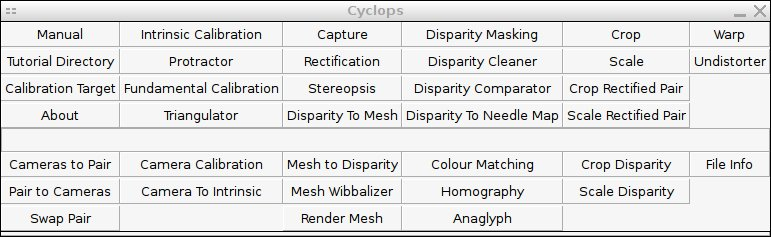
\includegraphics[width=0.9\textwidth]{screenshots/main_window}
 \vspace{-0.2cm}
 \caption{The Cyclops main window.}
 \label{fig:main_window}
\end{figure}  

Cyclops was originally going to be a camera calibration tool. It has since become somewhat bloated. Whilst its original purpose of calibrating cameras works perfectly well it has been extended to allow pairs of photos taken with calibrated cameras to be turned into 3D models, to be used for whatever purpose the user sees fit\footnote{It is preferred that purposes be evil. Maniacal laughter is not optional.}. It also has other uses, such as a tool for removing radial distortion from images and another for generating anaglyphs\footnote{I will try to explain everything I mention before this document draws to a close. All constructive criticisms should be sent to tom AT thaines $\cdot$ net. Non-constructive criticisms can be swallowed, whole.}.

This tool is primarily implemented for research purposes, but I have written this manual as though to an audience of relatively normal people. Whether this includes the humble reader or not is for the reader to determine. I have done this because the tool can make a very good demonstration of some technologies from Computer Vision, and so is of possible interest to other people. The background should never be forgotten however, this is not a user tested piece of professional software - it has bugs, inconsistencies and damned awful design. If you find yourself actually growing to like it I can only recommend the nearest suicide booth\footnote{May not be available in you area, era or reality.}.

On running the program a grid of buttons should be shown\footnote{If not shown then something has gone wrong. This is usually because the computer does not have GTK installed, you can confirm this by checking the log created when the program is run. To obtain GTK head to the GNU Image Manipulation Program website, www.gimp.org.}. Figure \ref{fig:main_window} shows this mess. Each button starts a mini-tool, each one is covered in detail by the chapter of the same name in the following document, with the exception of the four buttons in the top-first column. I leave the reader to work out what these do. Following this particular section an introduction to how it all works is provided, this is specifically for lay-people, but is still a bit of a head-full. The section following that, a pair of tutorials, is easy enough that anyone should be able to follow it. If the previous section knocks you off your feet this will hopefully pull you back up again. At the end of the document are three additional sections, the first covers general advice on capturing input for this tool, in other words what kind of input works well and what kind causes failure. The penultimate section is for those curious as to the technology used, whilst the final covers file formats for people who want to use Cyclops in collaboration with other tools.

 

\section{A Beginners Guide}

\begin{figure}[t]
 \centering
 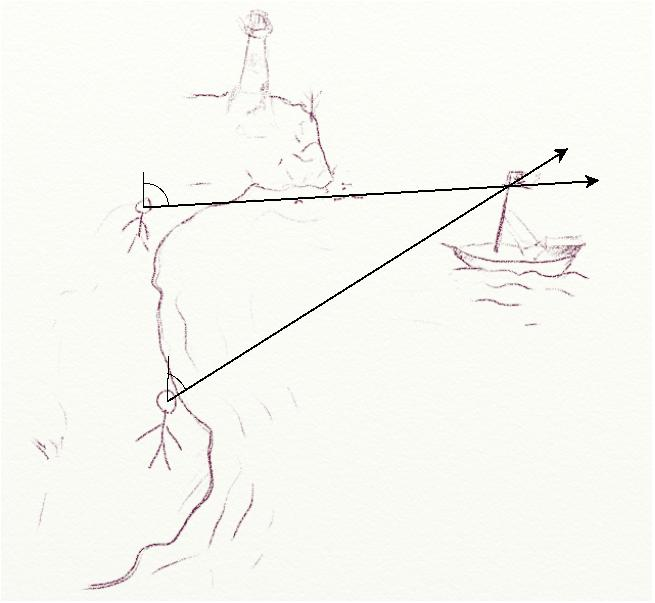
\includegraphics[width=0.55\textwidth]{diags/ship_map}
 \caption{Triangulating a ship by marking lines on a 'map'.}
 \label{fig:ship_map}
\end{figure}

Imagine that, whilst on the coast one day you see an anchored ship out to sea, and, not being entirely sure of your ability to guess, want to know where it is relative to the coastline.
In this day and age there are many ways of doing this, but having a compass, map, ruler and pencil handy you decide to do it yourself.
Standing on the coast you measure the bearing to the ship from your current position with the compass, you then identify where you are on your map and draw a line from that point with the recorded bearing. 
You now know the ship to be somewhere on that line. 
Walking down the coast some way you perform the same procedure, getting a different line. 
Where the two lines cross on your map is the ship, see fig. \ref{fig:ship_map}.

Being a particularly thorough person you then climb the nearby lighthouse and perform the same procedure again, expecting this third line to intersect at exactly the same spot.
It of course doesn't, but passes nearby where the other two meet.
There are several possible reasons for this:
\begin{itemize}
\item The boat could of moved whilst you were moving from measurement site to measurement site. This process necessarily assumes that the objects being measured don't change during the process of taking measurements.
\item North could of moved\footnote{Certainly not impossible, but if you want a more likely explanation then assume that the lighthouse is emitting a magnetic field.}, and with the calibration of the measuring device (compass) now being wrong the measurements will not be consistent.
\item Measurement error, the most likely explanation. When a boat is half a kilometre away a single degree out when reading the compass can shift it quite some distance.
\end{itemize}

The just described process is commonly known as triangulation.
Ultimately, triangulation is all that Cyclops is doing, plus a bit of device (camera) calibration, but there are some quite major differences between the two. I will now proceed to re-iterate how to solve this problem, three times, changing it slightly each time so it better maps onto the approach being used by Cyclops.

\begin{figure}[t]
 \centering
 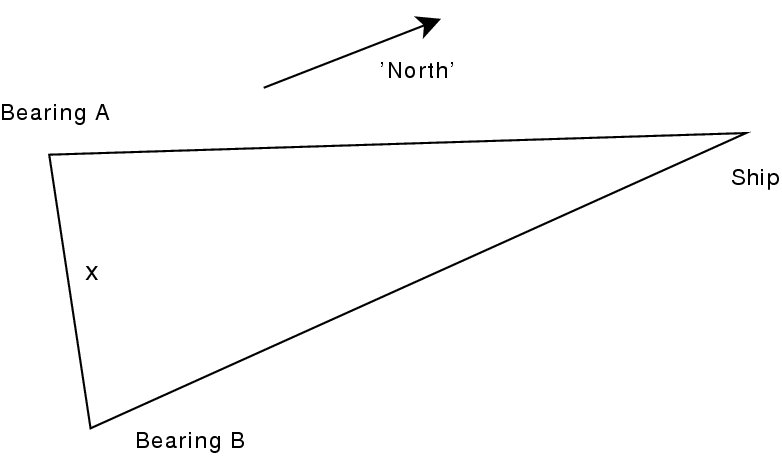
\includegraphics[width=0.55\textwidth]{diags/tri_map}
 \caption{A triangle.}
 \label{fig:tri_map}
\end{figure}

First, lets lose the map and draw our own.
That might look something like figure \ref{fig:tri_map}, otherwise known as a triangle.
The key points are:
\begin{itemize}
\item We have lost our position and orientation - we might know where the boat is relative to the two points we took measurements from, but we will not know where it is relative to any other features marked on the original map unless we apply the same procedure to those features. This is a fundamental restriction in what Cyclops can do. You can always run it multiple times such that the regions have shared features and match them up that way however. That is essentially how the map we had to start with would of been made in the first place.
\item The original map provided scale. In drawing our own we have lost this - we need to know the length of one of the triangles sides to know the length of any other side. The easiest side to measure in this case is the distance between the two measurement sites, but given a suitable range-finding device you could alternatively find the length of one of the other sides. If there were multiple ships and we had triangulated them all the distance between any two ships would suffice. More realistically, if we triangulated the front and back of a ship and knew its length that would also work. Cyclops suffers from this exact problem also, you don't get size unless you know at least one distance in the captured data.
\item The previous two issues are simple losses of information, they don't prevent you from doing triangulation. The final issue, which the sharp readers will have already spotted, is that we don't actually know the relative positions of the two measurement points. When previously using a map we could implicitly obtain this information, now we need to put some effort into calculating it. This is a relatively simple procedure however, you simply need the bearing from one of the measurement sites to another of the measurement sites. So you leave a marker, such as a stick in the sand, at your first position and when measuring at your second location take a bearing to the stick as well as to the boat.
\end{itemize}

\begin{figure}[t]
 \centering
 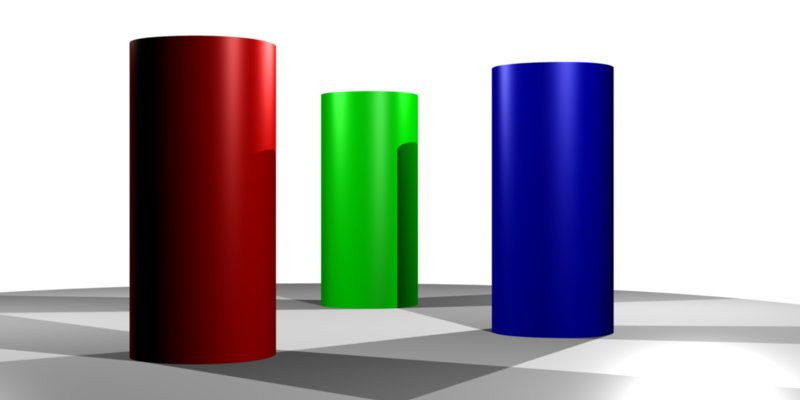
\includegraphics[width=0.45\textwidth]{diags/pillars_base} 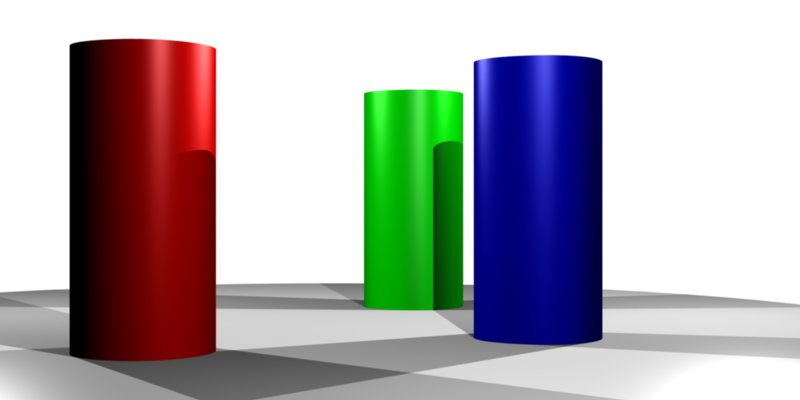
\includegraphics[width=0.45\textwidth]{diags/pillars_rotate}
 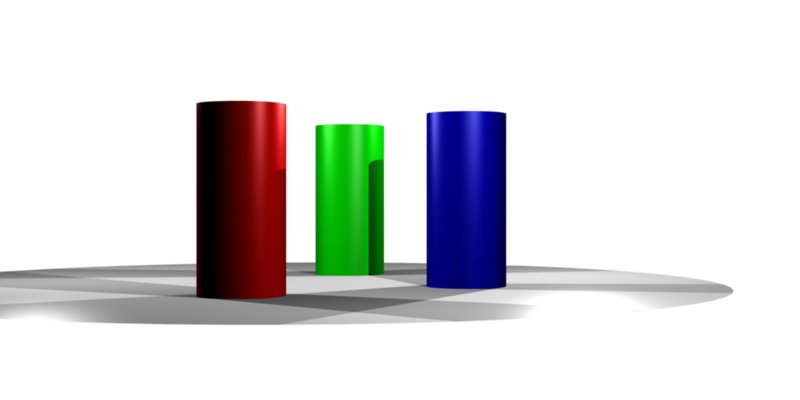
\includegraphics[width=0.45\textwidth]{diags/pillars_zoom}
 \caption{Three pillars from multiple views. You can work out your relative ($2D$) position easily. (Without using the pillar widths.)}
 \label{fig:pillars}
\end{figure}

By losing the map we have got a reasonably complete understanding of how Cyclops works, but now a further issue.
Compasses, with there universal north, can be rotated to get the bearing of any object you can see.
A camera does not have this luxury, the moment you rotate it, unless you match it up as you would do to create a panorama, you move to a different angular system.
This would mean that, following the previously described approach, you would always need to mark where the first photo was taken, and then take the second photo such that it can see the marker, possibly by constructing a panorama.
Ignoring panorama creation, which would require a tripod, simply marking where the first photo was taken in 3D space is far too tricky to do casually and is hence not an option.
So, for this scenario, we are going to pretend that no markers are available.
Solving this problem is not possible with a single boat, but imagine we have three boats to triangulate, or possibly three points on a single boat to triangulate.
With three points\footnote{They must not be on a single line, otherwise the calculation breaks down.} you can infer the relative angles of the cameras indirectly.
Unlike the previous steps, which anyone with a basic grasp of trigonometry could grasp, this is not so obvious.
To argue it I will use a simple mind game - imagine walking around three pillars on a circle, by looking at the pillars you can always determine your relative angle with and distance from the circle.
To aid your imagination figure \ref{fig:pillars} is provided.
So two (or more) views will by these three points know there relative positions.

For the final scenario imagine we don't have a compass.
This is easy enough to resolve; knowing north has simply been a proxy for taking angular differences, so its irrelevant as long as we can calculate these differences. We may do this by not moving the compass between readings at each measurement site. (As we are required to do with a camera anyway - see above.)
We still need a device with angles marked on it though.
In $2D$ this would be a protractor, using loci you could sit down and draw one on a piece of paper with some ingenuity; a little tricky but quite doable.
To move away from the example a little and talk about cameras we are going to need to turn a camera into the $3D$ equivalent of a protractor.
This requires a calibration step, such that we can work out the angles between arbitrary points on an image. Simply take it as writ that this may be done.


The previous paragraphs have described what Cyclops does in two dimensions. In three dimensions things get rather more complicated, but that is what Cyclops is there to automate. 
The correspondences between Cyclops and the above ideas are covered in the following list:
\begin{itemize}
\item The \emph{Triangulator} tool does triangulation. (Duh!)
\item The \emph{Fundamental Calibration} tool works out the relationship between two cameras using points in the scene. Unlike $2D$, where three points are required, in $3D$ seven points are required.
\item The \emph{Protractor} tool allows you to use a calibrated camera as a protractor.
\item Several of the tools allow you to calibrate a camera, but you will probably use the \emph{Intrinsic Calibration} tool to do it.
\end{itemize}
You should now have a rough idea of what Cyclops is doing, but the next step is to obviously try the tutorials in the next section.
There tutorials are independent of this, but you should have a better understanding of what is going on from reading this.



\section{Tutorial}
There are two tutorials within this section, and the next section (As well as many others) additionally takes on a tutorial form. If you have just read the preceding section then the first tutorial will be familiar as a direct application of the ideas given. The second tutorial makes use of greater automation and is significantly more complicated to understand, with more steps, though it involves far less overall (human) effort. I would not attempt the second tutorial before you have a complete understanding of the first. The following section describes intrinsic camera calibration, for the tutorials in this section input is provided with the relevant calibration information. If you want to capture and use your own input then the following section on intrinsic calibration will be necessary.


\subsection {Sparse Stereo}
To create a 3D model of a scene requires 3 steps:
\begin{itemize}
\item Capture two input images with calibrated cameras. (Can be, and usually is, the same camera.)
\item Calculate the relation between the two cameras, that is there relative positions and orientations.
\item Triangulate matched points from both images to get 3D coordinates. Polygons can then be constructed between the coordinates to create a mesh.
\end{itemize}


\subsubsection {Step 1}

Rather than asking you to go off with your camera and obtain a stereo pair this step has already been done for you. This has been done because calibrating a camera is rather a lot of work, and you don't necessarily have a camera to hand, so for a first attempt at using this tool it is easier to have the input ready. Additionally, there is some skill to taking stereo pairs that work well, so it's best to stick to input that is known to work for these first steps. You can find this stereo pair in the tutorial directory. (Hit the 'Tutorial Directory' button to bring it up.) You will find two images, labelled roofs-left.jpg and roofs-right.jpg, both taken with the same camera. There is additionally the file 'Canon EOS 350 50(80)mm.icd' - this is the calibration file for that camera. 

\begin{figure}
 \centering
 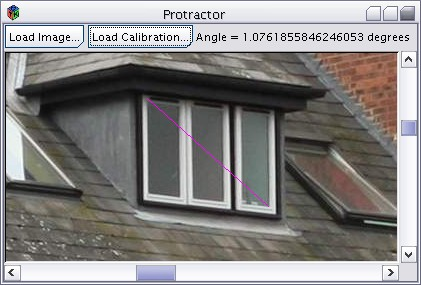
\includegraphics[width=0.75\textwidth]{screenshots/protractor}
 \caption{Screenshot of the protractor tool.}
 \label{fig:protractor}
\end{figure}

This is all the input you require for the next step. However, before moving on lets look at what the .icd file is actually doing. Click on the 'Protractor' tool, load either the left or right image and load the calibration file. You are now using the camera as a 2D protractor - see figure \ref{fig:protractor}. The angle measured is through the centre of the camera, you can think of it as measuring the angles between the light rays the camera captured. The end points of the pink line indicate the range of the measurement. To set the end points of the pink line either left click to snap the closest end point to the cursor or right click to alternate between setting the two end points to the cursors position.

A simple example of how this can be used directly is in measuring the height of a building.
You take a photo with the camera on the floor and measure your distance from the building, using the camera calibration you know the angle between the top and the bottom of the building.
You now have a right angled triangle and know a distance and an angle, simple trigonometry will hence give you the height of the building.
With some ingenuity and partial knowledge of a scene all sorts of distances can be inferred this way.


\subsubsection {Step 2}
We can now measure angles in our two photos, but this is not enough. To triangulate we also need to know the relative position and orientation of the camera when it took each photo. This next step obtains this information. I have in fact provided the output of this step as the file roofs.pcc in the tutorial directory, but you will learn nothing if you choose not to recreate this file yourself.

For this we need the 'Fundamental Calibration' tool, so load it up. First you need to load the two images. You will note that I label images left and right - this is just a convention, one image could be physically above another and upside-down for all it matters. The one thing that does matter is consistency, in this process we are going to create a .pcc file which is specific for two images - you can't latter swap the images around or use different images and expect it to work! So use the 'Load Left Image...' button to load 'tut/roofs-left.jpg' and the 'Load Right Image..' to load 'tut/roofs-right.jpg'. The images will appear - the left in the left pane, and the right in the right pane.

You now need to load the relevant .icd file for each image - this must match the camera the image was captured with. The two image were in fact captured with the same camera; I simply took one photo, took a sidestep to the right and then took the second. So load the 'Canon EOS 350 50(80)mm.icd' file for both the left images calibration and right images calibration.

We are now ready to calibrate, but don't hit the 'Calculate' button yet. Calibration requires a number of matched points to have been set, so hit the 'Add Match' button and click on a point in each image such that they are the same static location in the real world\footnote{That is, the points are the same bit of matter and that bit of matter hasn't moved between photos. If the two photos were taken simultaneously then any match would do. But if there is a delay then things that could of moved between shots should be avoided; trees swaying in the wind for instance. To further elaborate, what really matters is that the \emph{relative} positions of the matches stay the same, so you can in fact use moving objects, but only if you stick to one moving object alone for all steps and pretend that the rest of the scene isn't there. Boats make a good example of this situation.}. To calibrate requires a minimum of seven points, but to do a good job requires at least three times that. Additionally, the points you match should be widely dispersed around the images, as it won't work very well if they are all in one small area. As a final warning the points must not all be on the same flat surface - they must be distributed in 3D space. Doing this to a pair of pictures of a flat wall is impossible, but quite pointless as you should already know the shape of a \emph{flat} wall.

You will note that at any time you can click on the image and the nearest point to the mouse cursor will jump to the cursor, this can be used to refine positions, which is important as you ideally want to be pixel-perfect in your positioning. It also indicates which of the matched coordinates is selected by a different type of cross. If you want to select a cross without moving it you may right click, but the only thing you can do to the match is delete it, with the relevant button.

\begin{figure}
 \centering
 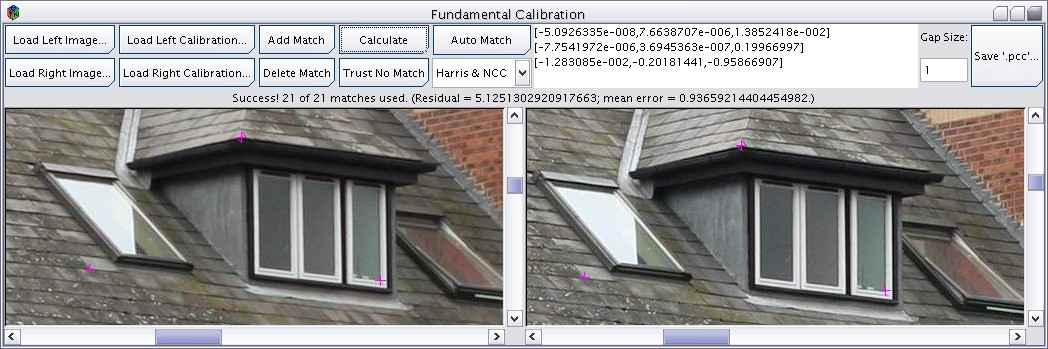
\includegraphics[width=1.0\textwidth]{screenshots/fundamental_manual.jpg}
 \caption{Screenshot of the fundamental calibration tool after Calculate has been hit.}
 \label{fig:fundamental_manual}
\end{figure}

Once you have enough matches you can click the 'Calculate' button - see figure \ref{fig:fundamental_manual} for what it looks like. For the moment you will always be using all the matches you have, the 'mean error' given is a measure of error - smaller is better, and you really want to be less than 2 for a reasonable result. However to get that requires pixel perfect positioning, so I wouldn't worry if you don't get that this first run through. The numbers that appear in the text box represent the fundamental matrix, if you know what this is then sweet, but otherwise ignore it. Just accept that calculating those numbers is the reason why you have been matching points for the last few minutes. If the mean error is too high you can keep adding matches and refine the positions of the matches you already have until its good enough for your tastes, just hit the 'Calculate' button each time you want an update.

And now for the final step - saving the .pcc file. Except there is one last piece of information we \emph{need} to know, the gap, which is how far apart the two cameras are in some unit of measurement. This is unknown however as the scene was photographed freehand. But ultimately, and fortunately, it doesn't really matter - all this does is scale the final 3d model, if we don't know it then we can't measure distances in the final output\footnote{Though we can measure relative distances - this wall is half as high as it is long, for instance.}. In reality it is far easier to simply leave gap as 1 and scale the model latter if you need to - take a tape measure with you and measure something in the captured images, or simply use an object of known size in the final output, scale it and problem solved\footnote{This is also far more accurate than measuring the distance between cameras, so is if anything the preferred method.}. So hit the save button and save that .pcc file - you can now use your own file or the file from the tut directory for the next and final step.


\subsubsection {Step 3}
We are now ready to make a 3D model, load up the Triangulator tool and have a look. You can probably guess what you need to do with the image loading buttons, the load calibration button will load the .pcc file. Once these three things have been loaded you can start triangulating - by clicking in the two panes you set a pink cross to indicate a location in each. When the two selected location match, i.e. are over the same real-world point the numbers in the top right will be providing useful information. It gives a 3D coordinate, this is from a coordinate system defined with the left camera at the origin pointing down the negative $Z$ axis. It also gives the distance from the centre of the left camera and the depth from the left cameras principal plane. You should also note the blue lines in both images, these are each calculated from the point in the other image and indicate where the point in this image must go to correctly match the other point (They are referred to as \emph{epipolar} lines.).

\begin{figure}
 \centering
 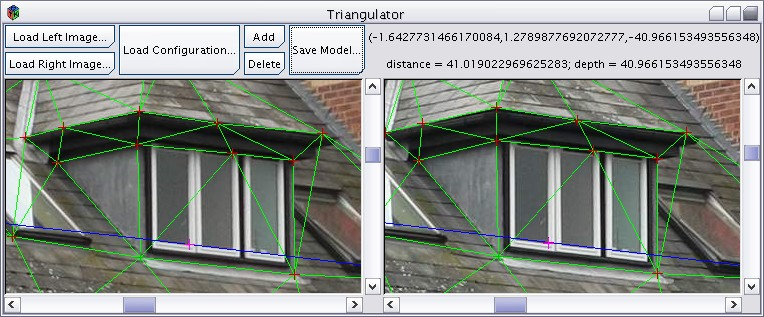
\includegraphics[width=1.0\textwidth]{screenshots/triangulator}
 \caption{Triangulation in progress - note how all the corners have been marked out.}
 \label{fig:triangulator}
\end{figure}

So we can now find the 3D coordinates of individual points in the image, but this is not exactly a 3D model. This is where the Add button comes in, you correctly match points, and then hit Add to store them. For each correctly matched point it creates a vertex in the resulting 3D model\footnote{If you want to delete a point you can right click to select and then hit the Delete button.}. It then automatically triangulates these vertices and allows you to save a mesh with the 'Save Model...' button. This outputs a wavefront file, a well known file format that most 3D modelling tools can handle. This file format includes UV coordinates for the left image, so that if textured with this file most modelling tools will automatically use the correct parts of the image for texturing. 

So go ahead, add a bunch of matches. It is not worth trying to do the entire scene at this point, so I would stick to doing a small area well. As you add and delete points the left and right panes will show a green mesh of triangles, these are a projection of the triangles that will make up the 3D model\footnote{It is a Delauney triangulation using the left image coordinates, for those who know what such a thing is.}. As each triangle is flat you should make sure that each triangle covers a flat piece of geometry, or a piece of geometry that can be acceptably approximated as flat. Corners should align with triangle edges to make sure they are sharp, you will often need to add extra vertices to make the triangulation do this. An inevitable consequence of occluding boundaries is that triangles you don't want will be created. Nothing can be done at this stage, they can be deleted from the 3D model latter. You can save a result out repeatedly and check it each time, so refinement is the order of the day. (See next section for visualisation.) The tutorial directory contains one possible output of this process, the file \emph{roofs.obj}. Ultimately, for the supplied input, you are triangulating an object that is $30*$ as far away as the baseline of the photos. It is extremely hard, if not impossible, for a human to get a model out that is not wonky using the limited tool-set provided. Generally, if you actually want to use the resulting model, you will clean it up in a 3D modelling program.


\subsubsection {Visualisation}
So, you completed all the previous steps to create a 3D model. But in a twisted turn of events you didn't actually get to see it, I left you dangling, with the expectation you would go and figure it out how to look at it yourself. This is probably a tad unfair, so I will now provide a quick tutorial on how to visualise this file in a completely free 3D modelling tool - Blender.

Blender is, in truth, like using a mallet to crack a nut - its far more powerful than our requirement to simply look at a 3D model. But its free (Open source) and available to download at www.blender.org, so go get a copy. If you have your own preferred tool then you can go and use that, this section is for those that do not already have experience in this area.

I am going to go for a button by button guide to doing this - I am using version 2.43, so if your version is different you might have to work out an equivalent. First you need to install blender, this should be as standard for your platform. Once installed run it, the default view should come up.

There are 3 sections to the screen, a menu bar at the top, a 3D view in the middle and a buttons bar at the bottom, where most of the functionality can be found. What we are doing is so simple that we can ignore the buttons bar for this tutorial. The 3D view will currently contain a cube, we don't want that so right click in it - a pink outline should appear to indicate that's its selected, hit the x key and confirm its erasure. Now we are currently in orthographic viewing mode - this is good for architectural drawings and the like, but not how we see, and not what we want here. Move your mouse cursor over the 3d view and hit the space bar - a menu will come up - goto the 'view' sub-menu and hit the 'Ortho/Perspective' button.

Now to load our 3D model, top right corner - hit the 'File' menu, go down to import and within that menu select 'Wavefront (.obj)' - use the file selector to find the file you saved from Cyclops and load it. When you hit load a menu will appear at the cursor - just hit ok - whatever you do don't move the mouse cursor off this without hitting ok, as that will cancel the operation.

You probably can't see anything - Blenders virtual camera is currently looking at the origin, which is where the camera for the original left photo is situated - the 3D model is somewhere off the top of the screen. We need to learn to navigate 3D space. All navigation is done with the middle mouse button, if you don't have one then holding down alt then using the left mouse button is the equivalent. The middle mouse button on its own tracks around the current view centre, you can also zoom by holding down Ctrl at the same time as the middle mouse button, if you have a mouse wheel then that also zooms. Shift plus the middle mouse button can be used to move. For now rotate down towards the bottom of the screen until you see the 3D model in the distance and right click it to select it. To save translating all the way over hit space and go to the view menu as previous, but this time hit the 'View Selected' button - this will snap you straight over to the mesh you have created.

You can now rotate around the mesh. This is where you will realise how bad a 3D model triangulated from two camera views from 20m away looks\footnote{The output from the second tutorial is far better.}. Especially when half the triangles are wrong. But regardless, you have something, and it would be nice if it was textured with the original photograph. In the 3d view there are a row of buttons at the bottom, in this is the mode selector - it will currently say 'Object Mode', make sure you have the mesh selected by right clicking on it and use it to flip to UV Face Select. Now hit the 'a' key, this is select all, to select all the faces. We now need to goto the UV editor window - on the same bar where the mode selector is there is a small drop down dialog as the first entry, which should show a grid pattern. This selects the type for the middle area, you will notice that the other two parts of the blender window also have these, its interface is insanely customisable. All we need to do is goto the 'UV/Image Editor', you should notice that various faces are selected in this view - these are the faces we just selected back in the 3d view. Now hit the 'Image' menu in the same place where the mode selector was, hit open and open the left roofs image, we have now assigned the texture so return to the 3D view. Once back in the 3D view return to object mode with the selector, this loses the nice texturing so then switch it back on using the drop down that is to the right of the mode selector to select 'Textured' from the Draw type selector.

\begin{figure}
 \centering
 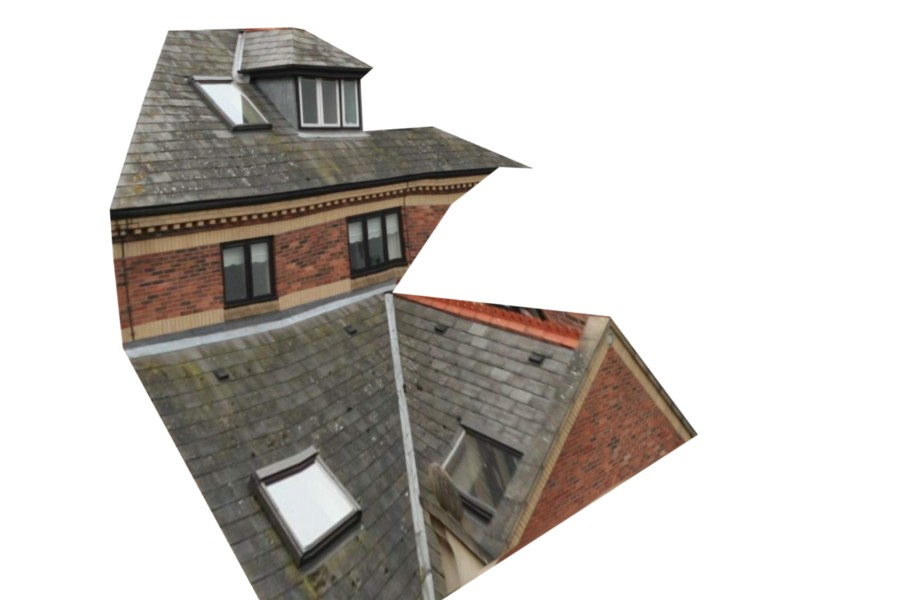
\includegraphics[width=0.7\textwidth]{screenshots/sparse_render}
 \caption{Render of a small chunk of the tutorial scene. Note that I have deleted several faces that were in the output as they were wrong. I have not however moved any vertices, which you would do if you wanted to actually use it.}
 \label{fig:sparse_render}
\end{figure}

You can now see your 3D model in all its glory. If you want to go further with blender have a look at the Blender website - www.blender.org, they have lots of tutorials, all better than this one. With a little work you can render up your mesh and clean it up as shown in figure \ref{fig:sparse_render}. The file \emph{roofs.blend} in the tutorial directory is the cleaned up version of \emph{roofs.obj} used to create the render in figure \ref{fig:sparse_render}. Blender also has extensive export options in the File menu, so if you use another tool that doesn't handle .obj files directly this will probably solve your problem.


\subsection {Dense Stereo}
Tutorial one is rather involving, requiring a fair amount of work to make anything substantial. Fortunately there is another way that requires far less effort from you, but far more effort from your processor - most of the steps in the previous tutorial can be automated by the computer. There are however more steps and more gotchas even though less actual effort is required by the human involved. Less effort, more skill you could say. 

The primary weakness of doing things the automated way is that it is considerably less robust, as whilst the human approach will nearly always work the automated approach can fail in ways that would be unclear to a user untrained in the intricacies of how it all works. Most critical is that a certain amount of knowledge is required to provide input that the computer can work with, and sometimes to recognise when it has failed before it becomes glaringly obvious.

Regardless of all the potential problems you will have to try before anything can go wrong. We will again be using the roofs stereo pair. The advantage of this is even more critical than for the first tutorial, as I can now put off explaining how to capture good data until section \ref{capture_advice}.


\subsubsection {Fundamental Calibration}
As in the previous tutorial we start with the \emph{Fundamental Calibration} tool. In fact, we require exactly the same file, the .pcc file, as was previously generated, and you could reuse the previously generated file or the one supplied. There is however a button that says \emph{Auto Match} in the interface, and we are now going to learn what it does. Use the four buttons on the left to load the images and calibration of the roofs image pair as before, then simply click the Auto Match button and wait. It will take a short while to run, during which you should notice the progress bar in the main window. If after this has run you scroll around the two image pairs you will notice that a lot of matches have been added, see figure \ref{fig:fundamental_auto}. If you now hit the \emph{Calculate} button it will do its stuff and you should get a good answer, in fact, nearly every time the result will be far better than you could ever obtain yourself. Save the file and your done.

\begin{figure}
 \centering
 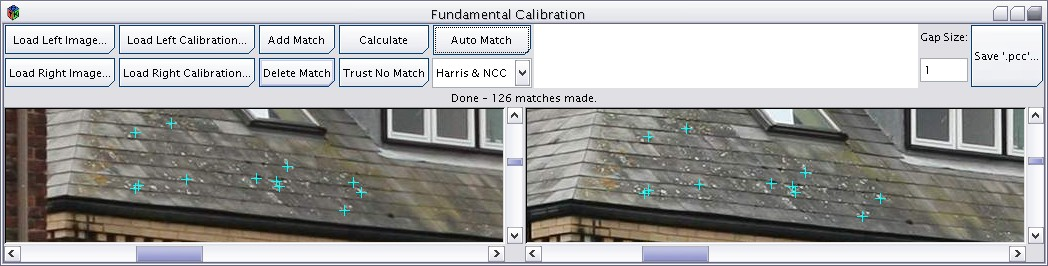
\includegraphics[width=1.0\textwidth]{screenshots/fundamental_auto}
 \caption{A set of auto matches that have found the bird shit to be a particularly good source of information. Sky rats are not entirely useless it seems.}
 \label{fig:fundamental_auto}
\end{figure}

\begin{figure}
 \centering
 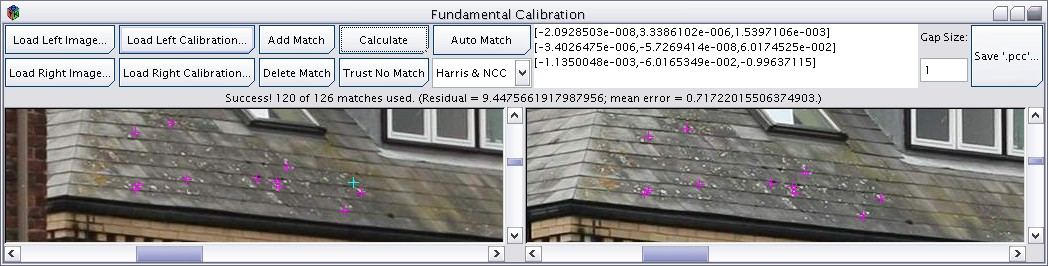
\includegraphics[width=1.0\textwidth]{screenshots/fundamental_result}
 \caption{The calibration view after the automatic matches have been used for calibration. Note the single sky-blue point in the left image that has been ignored, it is evidently bad.}
 \label{fig:fundamental_result}
\end{figure}

Before we move on however you might of noticed a difference from the previous approach - these matches are sky blue when the matches you did yourself previously were pink. And after it had calculated most of the matches turned pink, as in figure \ref{fig:fundamental_result}. This colour coding is an indication of reliability - pink matches are trusted completely, if any of them are wrong you will get a bad result. Sky blue matches are treated with suspicion however, and you can reasonably have half of them wrong and still get the correct answer. You do need a lot of them to make up for having less pink points however. After calculation all the matches that were used for the final result are set pink, so if you calculate again it will get an answer almost instantly.

The algorithm used is \emph{stochastic}, that is it uses random numbers, so each run you will get a very slight difference in how it gets to the result even though it will almost always get to the same result. Note the use of the word almost, it can fail. To recognise when this happens look at the number of matches used - if it isn't using at least half then you probably have a problem. You can also go around and check the matches it is using, if there wrong then the output is wrong. If this happens the \emph{Trust No Match} button should be hit, all matches will turn sky blue and be untrusted again. You can then hit \emph{Calculate} again and hope it works. Of course, if there are not enough matches or too many bad matches then it will never work and you will have to resort to doing it by hand.


\subsubsection {Rectification}
We now diverge from the manual approach entirely. Rectification involves absolutely no mental effort, you just hit the buttons and it works.

But before we do it some idea as to why it is done should prove useful, if only to satisfy any curiosity. When you use the \emph{Triangulator} tool it drew lines, refereed to as epipolar lines, such that for two points to be a valid match they must each land on the others epipolar line. Whilst not that useful for a human due to there exceptional matching capabilities this information is invaluable to a computer, as when trying to find a match in one image for a location in another it doesn't have to search the entire image - it only has to search along the one line. This can be integrated into the searching algorithm itself, but is easier to implement as an entirely separate step. Rectification is that step.

Rectification takes in an image pair and there corresponding configuration file, it then transforms all of them and allows you to write out a new set of files. The transformed versions are such that the previously mentioned epipolar lines are all horizontal and aligned. That is, a pixel at ($x_1$,$y$) in one image can only match a pixel at ($x_2$,$y$) in the second, so matched pixels must share the same $y$ coordinate. A simple examination of the two images output by this step should convince you of this, but if that is not enough just load them into the \emph{Triangulation} tool and look at the lines it draws\footnote{If the two points match and are not on each others epipolar line then the fundamental calibration step went wrong. This should be not be mistaken for noise in the calibration, where pixels can slightly diverge from the epipolar line because the calibration is not perfect.}.

Unfortunately this step will often make the images bigger. In fact, if you take one photo directly in front of another photo and then try this on them it will try to produce output that is infinitely large. For those of us who don't have infinite computers this tends to cause problems. It will also distort the images such that they are no longer square, so you will generally find a particularly garish pink border around your image, see figure \ref{fig:rectification}. This pink border is important, its the mask colour used by the program to indicate areas it should ignore\footnote{You can mask images this way yourself if you choose, to remove objects you don't like.}. The consequence of this is that after an image has been through rectification you can no longer store it in a lossy file, so do not use jpeg files. I personally stick to .bmp files, which is the default output for the rectification tool anyway.

\begin{figure}
 \centering
 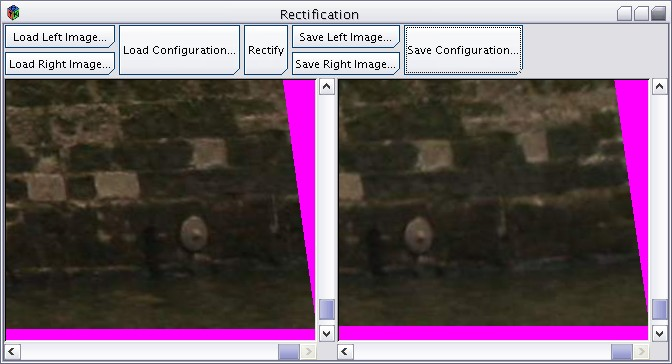
\includegraphics[width=0.7\textwidth]{screenshots/rectification}
 \caption{The rectification tool, post-rectification. This shows the pink border you usually get when rectifying.}
 \label{fig:rectification}
\end{figure}

So, time for a rectification; click the \emph{Rectification} button in the third column of the main window to bring it up. The buttons are fairly self explanatory, the first three on the left load the input, you then hit the \emph{Rectify} button and wait for the progress bar to jump along. When done and the two panes show your newly distorted images the final three buttons on the right can be used to save back out the new versions, which should then be used for the following steps\footnote{Be warned that the roofs pair when saved as .bmp files come to 30 meg each, so you will need 60 meg of storage for them. It will take a few seconds to write.}.


\subsubsection {Scaling and Cropping}
This step could be skipped but for practical reasons. The next step, \emph{Stereopsis} is the real resource eater of this entire process; if you think anything that has happened so far took a long time, or ate a lot of memory, your in for a shock. If you give it as input the data from the previous step it will take some time to run, eat lots of memory, and then, in a quite beautiful twist of fate, there will be so much data your graphics card will probably refuse to let you see the result\footnote{It can certainly be done, but it requires a lot more effort than is appropriate for a tutorial, so best to follow through here. The crux of it is using a geometry reduction tool to simplify things for visualisation. The alternative is to do Stereposis at high resolution and to then lower the resolution of the disparity map with the 'Scale Disparity' tool. This is the better approach as it will minimise noise in the output, at the cost of processing time and memory. In fact, you will require at least 2 gig of free ram to do the roofs pair at full resolution (A gig will do if you switch off smoothing.).}.

The lower the resolution of the input to the next step the faster it will run, for a first run you probably want to get it down to less than 500 pixels square, smaller if your computer is not very powerful. There are two ways to make an image smaller, you either scale it or crop it. Because the image pair is calibrated you can't just load the two images up in any old image editor and do this yourself, it has to be done consistently between the two images whilst also updating the .pcc file. In the fifth column of the main Cyclops window two promising buttons should reveal themselves - \emph{Crop Rectified Pair} and \emph{Scale Rectified Pair}. I'll let you choose what to do. Cropping is more interesting in my opinion as you will get more detail than if you scale the image to get the entire scene in low detail. You can do a combination of both in either order if you so choose.


\paragraph{Crop Rectified Pair}

\begin{figure}
 \centering
 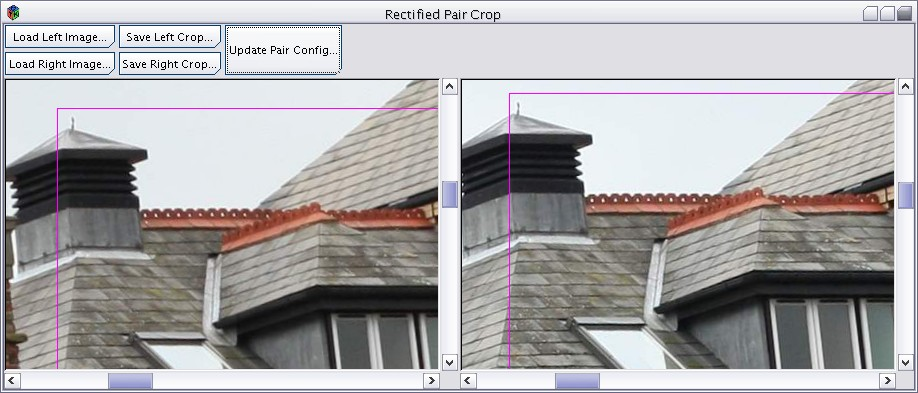
\includegraphics[width=0.9\textwidth]{screenshots/crop_pair}
 \caption{Cropping a rectified image pair.}
 \label{fig:crop_pair}
\end{figure}

The \emph{Crop Rectified Pair} tool is mostly self explanatory, the steps are as follows:
\begin{itemize}
\item Use the two left hand buttons to load the image pair.
\item Set the pink boxes to cover the region you want, obviously for it to work the regions must cover the same object. Left clicking will jump the nearest corner in the image to the mouse cursor whilst right clicking will centre the box with a size of one pixel where you click. Generally, to set the boxes you will first right click in the centre of whatever region you want in both images, then by left clicking expand the region out and refine to your desire. You will note that the top and bottom of the boxes in the two images will always align with each other, to maintain a valid rectification.
\item Once done do not edit the boxes and save out the results using the three remaining buttons to create a new triplet. The \emph{Update Pair Config...} button works by first asking you for the original file, which it loads and updates, before asking you where to write the new version.
\end{itemize}


\paragraph {Scale Rectified Pair}

\begin{figure}
 \centering
 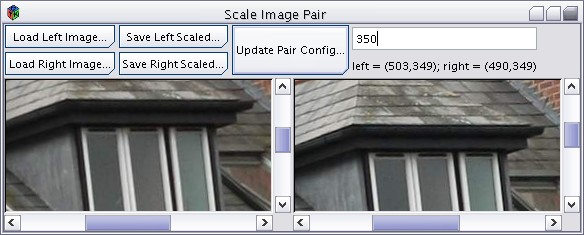
\includegraphics[width=0.6\textwidth]{screenshots/scale_pair}
 \caption{Scaling a rectified image pair.}
 \label{fig:scale_pair}
\end{figure}

Just like cropping, this tool is again mostly obvious. In fact, its use is identical to cropping except you edit the height of the images rather than set boxes:
\begin{itemize}
\item Use the two left hand buttons to load the image pair.
\item Edit the single text entry box to change the vertical resolution of the images, it will show the new dimensions of the images below.
\item Once done save out the results using the three remaining buttons to create a new triplet. The \emph{Update Pair Config...} button works by first asking you for the original file, which it loads and updates, before asking you where to write the new version.
\end{itemize}


\subsubsection {Stereopsis}
The Stereopsis tool is a perfect example of something that is really easy to use, but has an implementation that belongs only in nightmares. I will first instruct you on getting the Stereopsis tool going, I will then explain what it is actually achieving before finally telling you what to do when it has finished. The idea is that whilst it does its thing you can continue reading this tutorial.

You should know the pattern by now - we have three files, the two images and the .pcc file. Previously we have edited them with various operations, now we are going to create a fourth file. For this we in fact only need the two images, the .pcc file is irrelevant for this step, though required again to make a 3D model. The two buttons on the left are the only clue you should need, so load the two rectified images to get something like figure \ref{fig:stereo_before} and hit Run. That is it, now you wait.

\begin{figure}
 \centering
 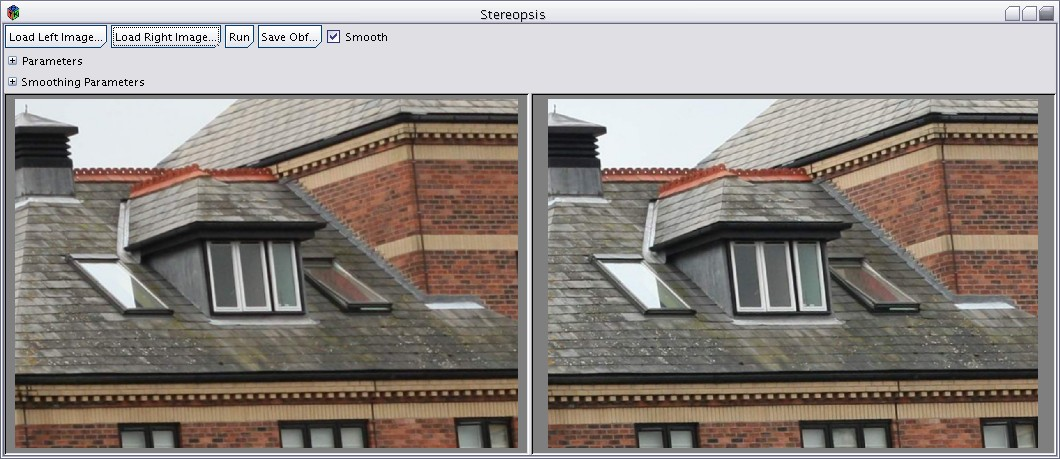
\includegraphics[width=1.0\textwidth]{screenshots/stereo_before}
 \caption{The Stereopsis tool, before being run.}
 \label{fig:stereo_before}
\end{figure}

If you followed my instructions with regards to scaling and cropping then it won't actually take too long, but here is as good a place to insert information on what is happening as any. As previously discussed, the images have been deformed such that pixels can only match pixels on the same scanline, this tool will now find those matches. These are represented as a \emph{disparity map}. This map is simply an image of offsets on the x axis such that if you take the left image, take each pixel from it and move it by its value from the disparity map you should end up with an approximation of the right image. Of course, some parts of the left image are not visible in the right image and vice-versa, so there will be gaps. Now this is something us humans do all the time - you are doing it now whilst you read this document. But computers find this hard, really hard in fact, and whilst everything else provided by Cyclops is basically stable technology stereopsis is an area of continuing research explored by hundreds of scientists world-wide. The algorithm provided is reasonably good, and, importantly, easy to use\footnote{It does have parameters you can set, but it is probably not worth touching them, though increasing the Occlusion Cost parameter can reduce noise at the expense of losing detail. This is actually quite unusual, most stereopsis algorithms have parameter that need fine tuning for each individual image pair.}.

\begin{figure}
 \centering
 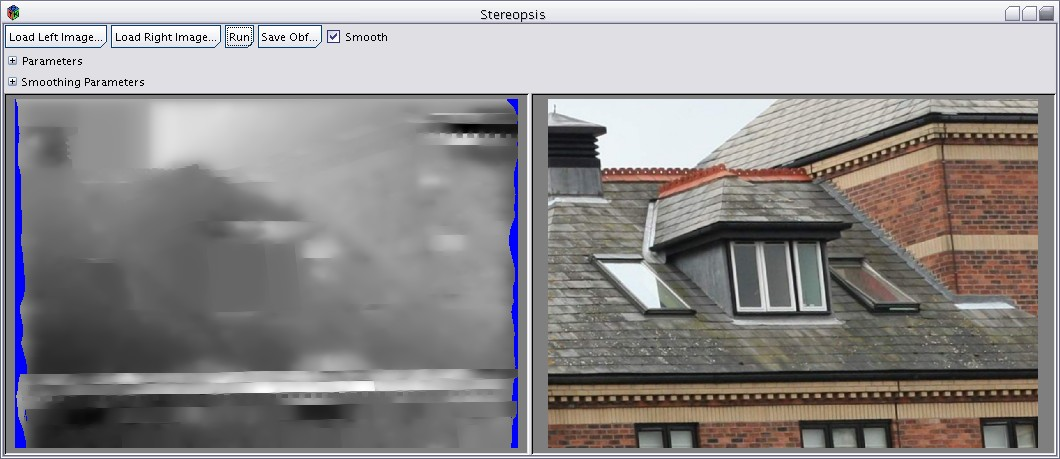
\includegraphics[width=1.0\textwidth]{screenshots/stereo_after}
 \caption{The Stereopsis tool, after being run.}
 \label{fig:stereo_after}
\end{figure}

When it has finished running the left image will be replaced with the calculated disparity map as in figure \ref{fig:stereo_after}. You should get a sense of depth looking at this, depending on the camera configuration white will represent either close objects or distant objects and black the other, with shades of grey in between. Use the \emph{Save Disparity...} button to save the disparity map for future steps.


\subsubsection {Warping}
This section is entirely skip-able, but worth doing as it will show you precisely what the output of the last step is. This involves the \emph{Warp} tool, found at the top of the sixth column of the main window; run it.

\begin{figure}
 \centering
 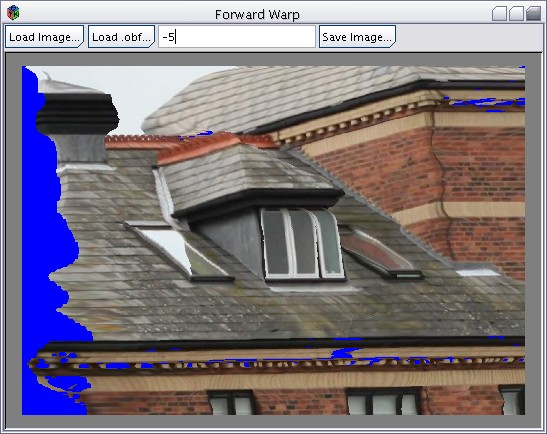
\includegraphics[width=0.6\textwidth]{screenshots/warp}
 \caption{The warping tool, with a particularly extreme value to show how far it distorts in such cases.}
 \label{fig:warp}
\end{figure}

With the \emph{Load Image...} button load the \emph{left} image of the rectified pair; with the \emph{Load Disparity...} button load the saved disparity map. The image area will now show something that, all being well, should be reasonably close to the right image. There will be various blue patches that indicate areas where no information is available, but if you compare the two it should mostly be a good match. The number at the top indicates a multiplier for the disparity maps offset, if you set it to 0 you will get precisely the left image. Setting it anywhere between 0 and 1 will interpolate between the left and right image. You can also set it outside the$[0,1]$ range, but the further out you get the greater the distortion, see figure \ref{fig:warp}.

That's it, trying various numbers is all I want you to do. You can save the generated image for the current number with the \emph{Save Image} button if you want. If your particularly patient and have a tool to stitch together images into an animation\footnote{Blender will do it.} you can produce a whole set of images and create an animation, which can be quite cool\footnote{Using a sin wave for the parameter and making the animation cyclic so it bounces backwards and forwards can be particularly sweet. If you really care about this you might want to look at the Super Warp tool, which has this built in.}.


\subsubsection {Disparity to Mesh}

\begin{figure}
 \centering
 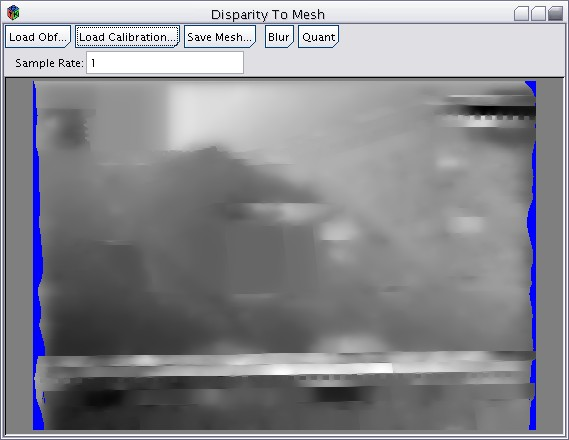
\includegraphics[width=0.7\textwidth]{screenshots/disparity_to_mesh}
 \caption{The disparity to mesh tool..}
 \label{fig:disp_mesh}
\end{figure}

Warping looks good, but a 3D model is where the action is. This is where the \emph{Disparity To Mesh} tool, found at the bottom of the third column of the main window, comes in. You do not actually need either image, you load the disparity and the calibration files and then save a mesh. That is it, see figure \ref{fig:disp_mesh}. This by default outputs a .ply file, which is different from the .obj files that the triangulator will write, if you want a .obj file simply give the file name .obj as its extension\footnote{.obj files are more consistently supported, problem is they are not very efficient as they are text files. Ply files can be binary on the other hand, making them far smaller than equivalent .obj files. This doesn't matter so much for the triangulator as no human is ever going to produce that many vertices. This outputs a vertex for each pixel however, making .obj files rather impractical.}. Viewing the 3d model is again left up to you, thought the same instructions work as for the first tutorial for using Blender\footnote{Except you should be using the .ply importer rather than the .obj importer. Unfortunately at the time of writing the Blender .ply importer (and exporter) are partially broken. The fixes are relatively minor however, and fixed versions are available on my website. Be warned that it is very slow and extremely memory consuming. (The code, not my fixes. To fix this would be a re-write.)}.


\subsubsection {Final Words}

\begin{figure}
 \centering
 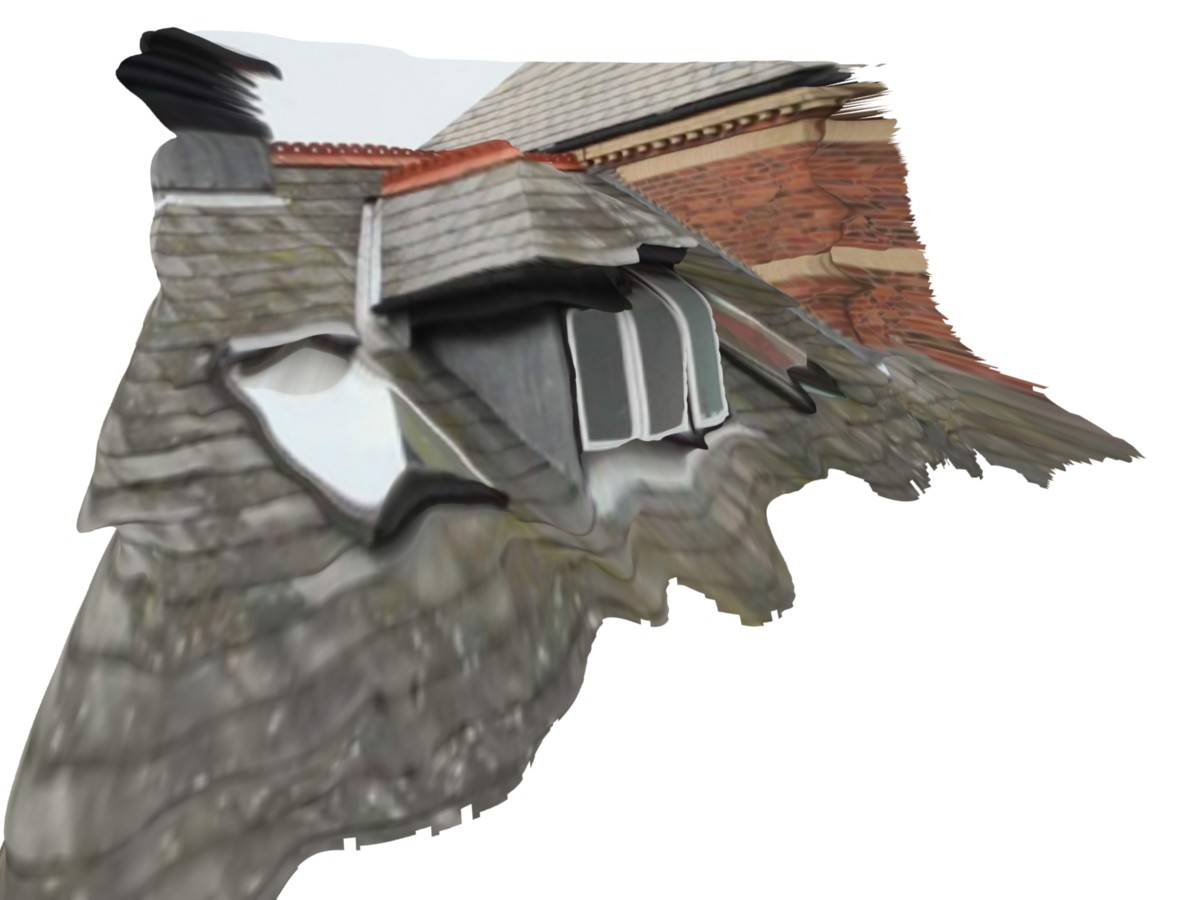
\includegraphics[width=1.0\textwidth]{screenshots/dense_render}
 \caption{A jelly-like render of a possible final output. As the resolution is quite low the quality is not that good. Higher resolution brings higher quality. I did delete some polygons from the edges, edge regions tend to be a problem due to not having anything to match to.}
 \label{fig:dense_render}
\end{figure}

With a bit of luck you should have now created a 3D model from a pair of images, such as the rendering in \ref{fig:dense_render}. The next section will give you the relevant information to calibrate you own camera, so you can take your own photos and make 3D models of your own. Note however that this section has relied very heavily on the input provided being the correct kind of input, section \ref{capture_advice} contains information on how to capture the correct kind of input, and would be recommended reading to avoid the disappointment of it not working when you try it yourself.

To keep this section relatively simple I have omitted many methods that can be used to improve the results.
The most valuable are the \emph{Disparity Masker} tool, which can be used to remove bad/unwanted (i.e. sky) regions, and the \emph{Disparity Cleaner} tool, which can remove noise from the disparity map and fill in the gaps.
Scaling Disparity maps rather than rectified image pairs takes longer because of Stereopsis, but is definitely preferred.
The \emph{Crop Disparity} and \emph{Scale Disparity} tools allow this approach to be taken.
Parameter tuning the Stereopsis algorithm can also improve the output, and applying the \emph{Colour Matching} tool prior to Stereopsis can improve the results in some situations dramatically.
These tools are documented in the following manual, taking the time to learn them is well advised if you intend to use this tool more than once, as the difference there correct use can make is spectacular.

It should also be noted that Cyclops can do things not covered by the tutorials here. Of interest to the amateur are the \emph{Homography} tool, a somewhat divorced helper for extracting textures from photographs, and the \emph{Anaglyph} tool, which allows for the easy creation of images that look 3D when viewed with the correctly coloured glasses. Further to that read this manual, as it details what each tool is capable of; you may then chain them together to solve a slightly more expansive problem set than indicated here.


\section{Intrinsic Calibration}
\label{intrinsic_calib}
If you have just completed one or both of the above tutorials and now want to use input captured with your own camera then you have come to the right place. Before we get onto a tutorial on how to use this tool an understanding of calibration in general is required, so below are some general notes. After that is a tutorial and following that a \emph{by the buttons} guide to this tool.

\subsection{Notes on calibration}
Firstly, realise that there are multiple ways to calibrate a camera. This techneque works as such:
\begin{itemize}
\item You obtain a 2D calibration target. Because its 2D and also because scale doesn't matter you can just print it out of any desktop printer.
\item You take a number of photos of the target, for this you need at least 4, I usually use twice that but take even more photos still in case some turn out to be out of focus. In general, more is better as it will do a better job, but it takes longer to process with each added photo.
\item The photos are loaded onto the computer the usual way.
\item Each photo is loaded into the Intrinsic Calibration tool and the user positions the virtual calibration grid to match the actual calibration grid.
\item The user hits Calculate, if it isn't set to \emph{Low} they then go off and have tea or something whilst they wait for it to finish.
\item The .icd file is saved. 3D models are created. Everyone rejoices.
\end{itemize}
The advantage of this method is the 2D calibration target, as printing is easy, the disadvantage is needing multiple photos. Cyclops also has another tool that will do the same thing, the 'Camera Calibration' tool. This requires only one photo, but the calibration target has to be 3D. There are also other ways of doing it. This method has an advantage over all the others however in that its very easy to give it lots of information, and more information generally leads to a better result.

If the above sounds like it takes a lot of work, then, well it does. In fact, it involves some very repetitive clicking to do well, so you have to be on the lookout for RSI\footnote{Repetitive Strain Injury. This is caused by, well, repetitive motions, such as lots of clicking with a mouse. If it gets you, stop, save what you are doing, and have a break. It only gets worse if you ignore it.}. Fortunately you only have to calibrate each zoom level on each camera once\footnote{Unless you can change lenses, in which case each zoom level on each lens for each camera.}. Well, that's the practical approach. Truth is, near enough everything changes a cameras calibration, from its focal length (zoom), aperture (f-stop), depth of field, temperature, age and probably some other stuff. But because its so hard to calibrate and there are so many other sources of error in the system going to such efforts is hardly justified.

A certain degree of accuracy is required. The first mistake you can make is when you hit the print button - those squares on that calibration target are meant to be square, if there not it just won't work. So make sure your printer is not going to change the aspect ratio. Default setting really shouldn't, but I am yet to encounter a printer manufacturer that I would trust, even when talking about something so simple. The calibration target is also meant to be flat, so don't bend the paper at all. The ideal is to stick it in a picture frame, but as devoting a picture frame to a printout of some squares is a tad strange its probably advisable to stick to keeping it between heavy books when its not in use. Or, as its such a rare occurrence to calibrate a camera, print out a new one each time, though paper costs trees and ink appears to be more expensive than gold bullion, so I prefer to avoid that.

Given that you have got the target right you now need to get the camera right. The basic rule of thumb applies here - you get what you pay for. The more expensive cameras are mostly better for this stuff, but you can still get perfectly good results from a cheap compact, and in truth unless your reasonably experienced at doing this you are going to cause more problems than your camera. Next issue is zoom - its got to be the same level of zoom when you take each photo for calibration, and the same again whenever you take a photo to use with the resulting calibration. This basically means that with a zoom lens you only have two usable zoom settings - out as far as possible and in as far as possible, as other setting can't be accurately recreated. If you got one of those cameras with a 10x zoom your basically down to one level anyway as zoomed right in will prove useless\footnote{Actually, the larger the zoom range of the camera the more distortion you will get. The cameras that advertise crazy zoom ranges are the worst to be using with this program, as there full in zoom is useless and there full out comes with so much distortion that Cyclops struggles to cope. The best lens to use is a prime, that is a lens with only one fixed zoom level, but that option is only available to people with SLRs and money to burn.}.

So, you have the equipment, now its time to take the photos. All you need is four, ideally more, I recommend eight. The photos should have the following properties:
\begin{itemize}
\item The target is wholly included in each photo, such that you can accurately locate the corners of each of the 256 squares. This is harder than it sounds. The issue is one of focus - the ideal photo set will mostly have the target filling the majority of the image with some at a steep angle to the target such that the target covers a large relative depth range. This will push the camera to the limits, especially as a lot of cameras have problems focusing on an object such as the supplied calibration target. The trick is to simply take twice as many as you need and only use the photos that come out right!
\item You can accurately locate the corners of \emph{all} the squares. This means photos that are sharp (i.e. in focus - see above.) with a large contrast. Make sure the target is well illuminated and not shadowed in any way. You can use a flash, but automatic focusing works best with a well lit scene, so best avoided really.
\item The photos are all at random angles with the target in different positions and orientations with the frame. Whatever you do don't try to follow some kind of pattern, use a tripod or do anything that will remove that random element.
\end{itemize}
To give an idea of what a good set looks like the photos I calibrated the lens/camera I used for all the sample photos is in figure \ref{fig:calib_images}.

\begin{figure}
 \centering
 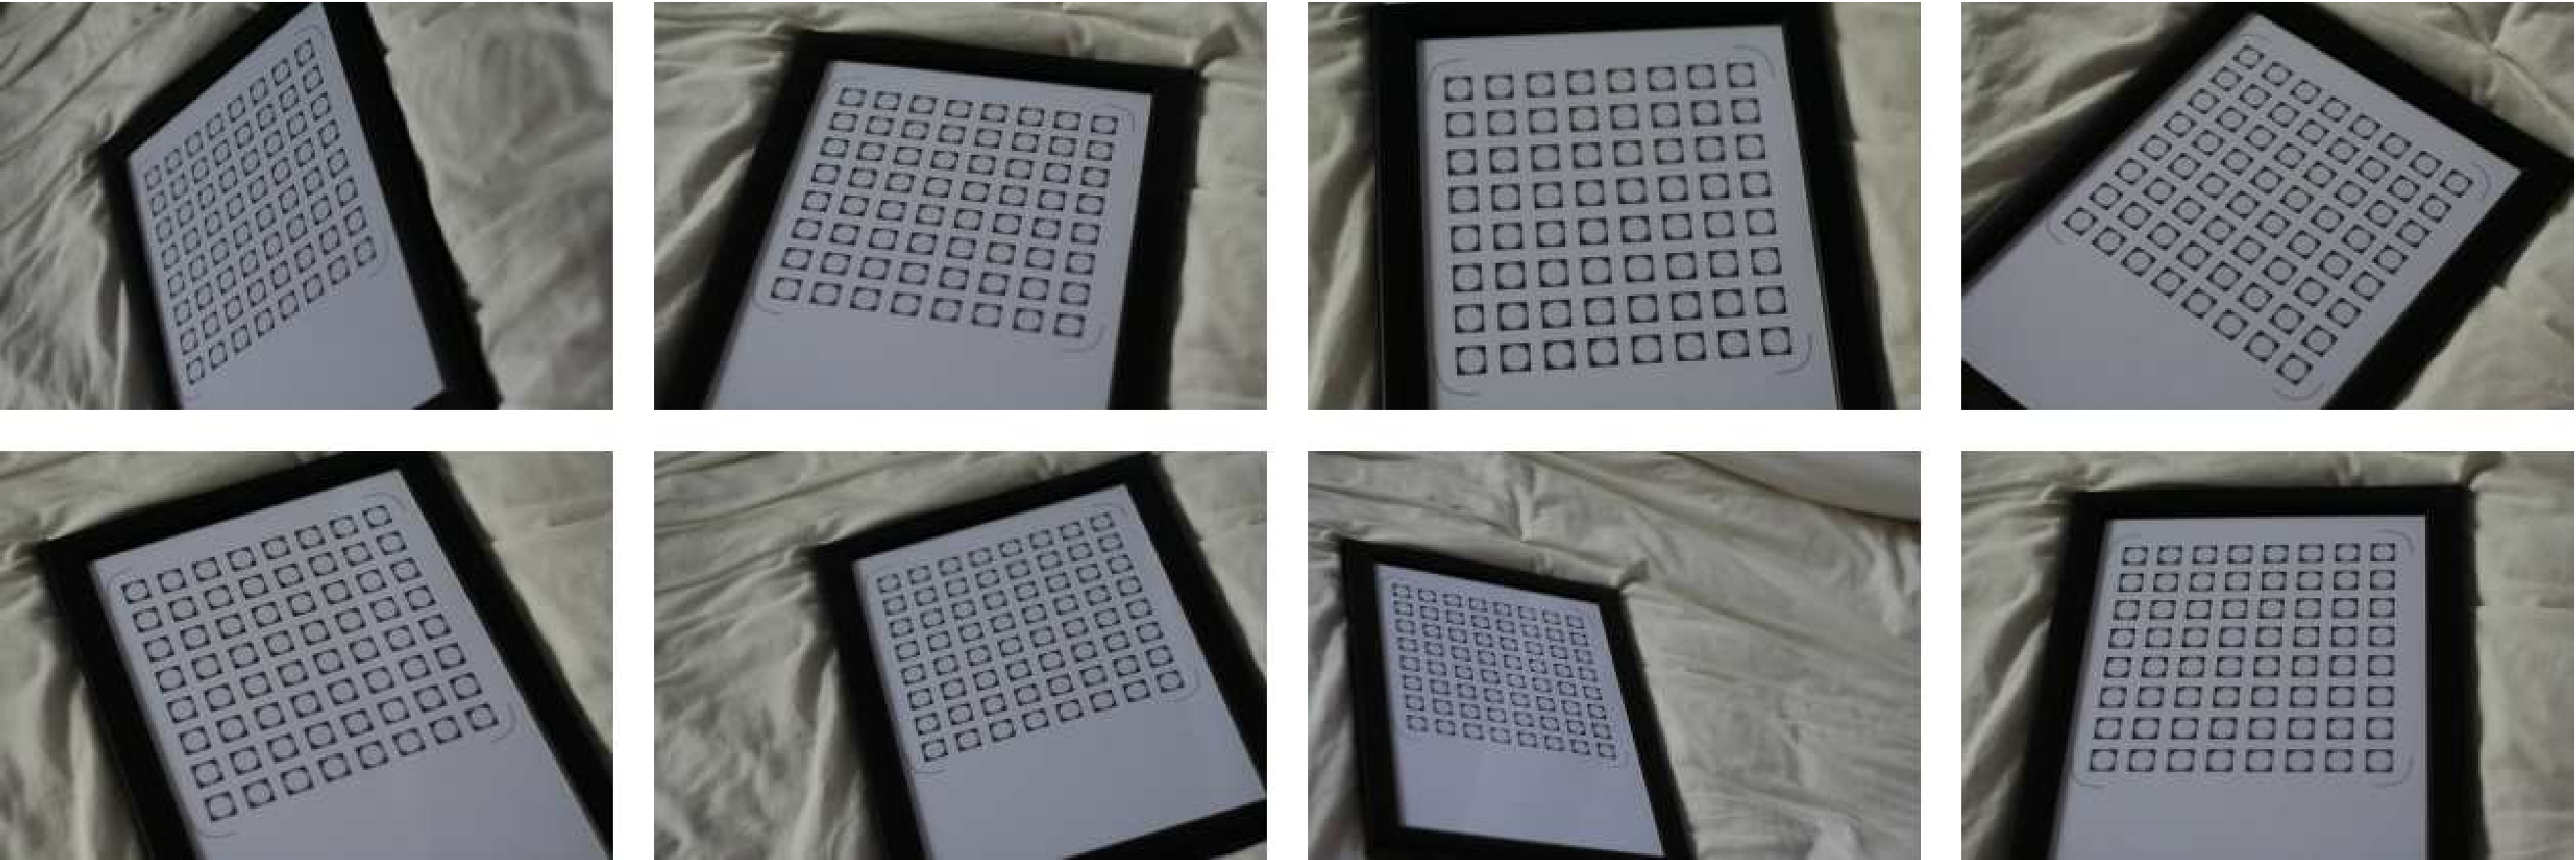
\includegraphics[width=1.0\textwidth]{screenshots/calib_images}
 \caption{A set of 8 photos, as used to calibrate a 50mm lens attached to a Canon EOS 350 with which I took all the example photos provided. (The EOS 350 has a 1.6 multiplier, so the lens is actually a 80mm lens when used with this camera.}
 \label{fig:calib_images}
\end{figure}


\subsection{Tutorial}

I am going to presume you have \emph{read} the previous sub-section and know how to take a set of photos, how many you want etc. So do it. I'm not providing input for this, as if you have not given up at this point you will most definitely want to use your own camera anyway. If you haven't guessed, the 'Calibration Target' button should open the .pdf file that you should be printing, otherwise you can find it in the programs doc subdirectory.

Once you have the photos on your computer in a format that Cyclops understands (Jpegs work fine.) hit the 'Intrinsic Calibration' button to bring up the relevant tool. Calibration is three step at this point:
\begin{itemize}
\item Use the add shot button for each shot and align a virtual version of the calibration target with the real one in the image, this is the fiddly part.
\item Select the quality level you want, hit 'Calculate', wait.
\item Use the 'Save .icd' button to save the calibration file. You can then go back and do one of the tutorials with your own input.
\end{itemize}

\begin{figure}
 \centering
 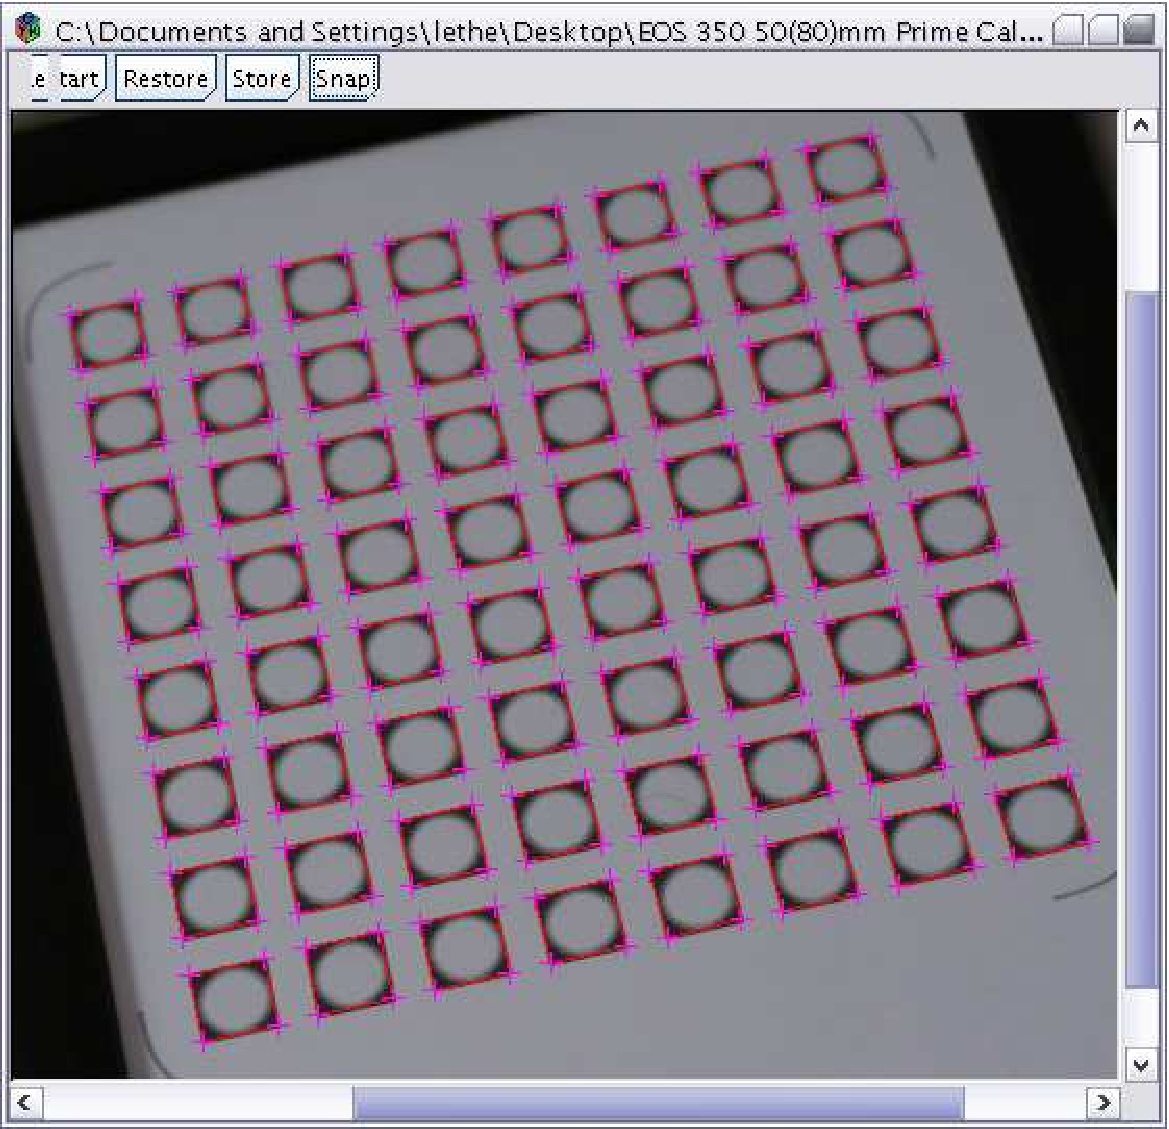
\includegraphics[width=0.7\textwidth]{screenshots/calib_grid}
 \caption{A calibration grid after the 4 corners have been set. Note that I shrunk the image down to make this screen shot, in reality most cameras produce far larger images so scrolling is involved.}
 \label{fig:calib_grid}
\end{figure}

The 'Add Shot...' button brings up an open dialog for you to open an image, select one of your images and hit Load; the open dialog is replaced with the image itself in a window and several buttons. When you first load an image you are in a helper mode which expects you to click on the image 4 times with the left mouse button - once for each of the 4 outer corners of the 4 corner squares. Given these 4 coordinates it can get the rest of the points in roughly the right position to make the next steps easier. So do this, go around the square (Clockwise or anti-clockwise.) and click on the 4 corners, but be accurate - doing a good job now can save latter work. If you screw up just hit the restart button and start again. When done you should have something like figure \ref{fig:calib_grid}.

To get a good calibration you need those red squares to align with the squares in the photo, after those 4 clicks it will have got it close, but not perfect. If you click on the image near a point it will jump to the cursor, you can also drag. This allows you to accurately line them up by hand. This is rather tedious, and frankly a health risk, so just hit the 'Snap' button, wait a bit, and watch as it does it for you. This works most of the time if the photo is sharp, but it will occasionally make mistakes, and if the photo is de-focused even slightly it will get it wrong. So you will need to go over the image and refine it as needed, if your lucky you might not need to do a single edit, but if the lens has a tight focal range that you can't get around you might end up doing a large chunk manually. In such situations the 'Store' button is invaluable, as it allows you to save progress so you can come back and finish latter. It creates a file in the same place as the image loaded, the next time you open the file in Cyclops instead of it going into the helper mode it will already be setup, with the points where they were when you last hit Store. You can also revert to the last stored set by hitting Restore. When you have multiple images open the 'Store All' button in the main intrinsic calibration window works exactly as you would expect.

\begin{figure}
 \centering
 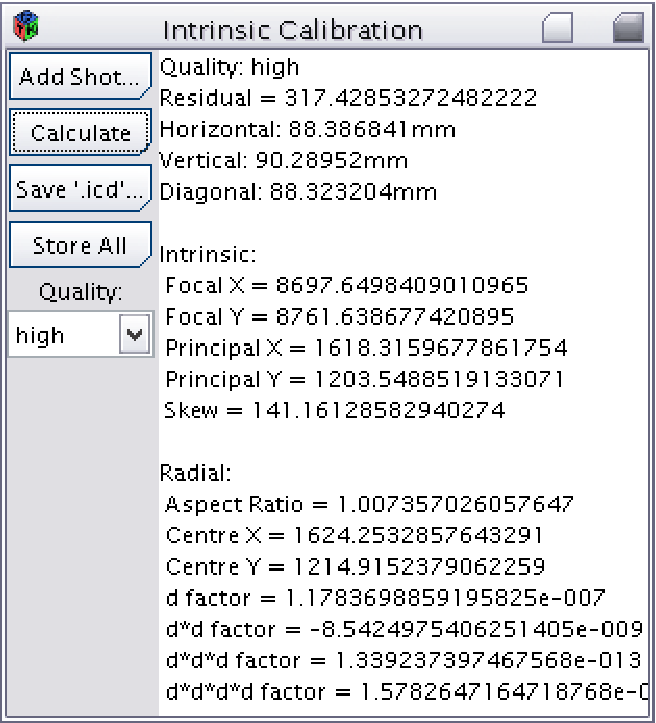
\includegraphics[width=0.5\textwidth]{screenshots/calib_end}
 \caption{The main calibration window after calibration has been done.}
 \label{fig:calib_done}
\end{figure}

You need to load in and perform the above on all the images in your data set, for a first run you might want to just do 4, its easy enough to add more latter and hit 'Calculate' again. Before you do hit 'Calculate' set the Quality to low, then hit that button - it will take a split second and the white area will fill with various numbers. These will be mostly meaningless unless you know about cameras in a mathematical sense, but three of them can be used as a sanity check. Specifically, the Horizontal, Vertical and Diagonal entries near the top - these are 35mm equivalent focal lengths calculated in 3 different ways, which your camera will give you, often on the barrel of the lens. One would therefore hope that all three values match the value your camera gives. In truth they won't, but they should be reasonably close. The manufacture stated values can be as much as 15\% out though, for instance figure \ref{fig:calib_done} shows my 50mm lens, which should be 80mm on the given camera, but instead I get 90mm. That is an error of 9.4\%, though the actual error in the lens is 5.9\% because of the 1.6 focal multiplier of the camera. The reason for providing 3 values is because there is no correct way of giving a 35mm equivalent focal length for a camera that is 3:4, which most compacts are, so different manufactures calculate it in different ways, hence the multiple values. For a professional camera that is 2:3 all 3 values should be about the same.

Low quality is not very good, it will work fine, its just exceedingly easy to do better. You want to set it higher, so head for a Quality of normal\footnote{If your wondering about setting it to high its frankly pointless, as any accuracy gained here beyond normal will be lost in other steps. It also takes twice as long, but then again, I always use high myself, but that's mostly because I sat down and expended time adding that option. I like to \emph{pretend} it was worth it.} and run it again. This will take a while, if your computer is particularly feeble and you have given it a lot of images you might as well go and put the kettle on. You may now save the .icd, and start capturing your own input. Though you might want to read section \ref{capture_advice} first, as there is a certain knack to taking stereo pairs.


\subsection{By the Button}
The Intrinsic Calibration tool consists of two window types, one control window and multiple image windows. When done calibrating close the control window and, after confirmation, it will remove all its associated image windows as well. Following the same convention you may remove an image from the calibration by closing its associated image window.

The control window, headed \emph{Intrinsic Calibration}, has two sections, a set of four buttons and a quality selector on the left; a results viewing area on the right. The first button adds a new image to the calibration, you first select the image file and, assuming Cyclops can open it, then it will appear in a new image window. The second button uses the currently selected quality level to \emph{Calculate} the calibration. You must have added at least four images before this will work, and unless quality is low it will take time, during which the progress bar in the main Cyclops window will do its job. The results area is blank until you have hit calculate, after which it will display information about the most recent calibration. Some of this information can be used to verify that the process has worked, but most people will mostly ignore this information. The third button allows you to save the calibration to be loaded by other tools. The \emph{Store All} button stores the calibration grid for all currently open images. This means that when you re-open each of these images it will also reload your work in fitting the calibration grid. This is good for having a break if RSI is getting to you.

Each image window is titled by the images file name with a header of four buttons and the image below. Unfortunately no zooming is supported, so you will usually have to scroll around the image. When you first load an image without a stored calibration grid or after hitting the reset button you are in a special mode to quickly place the approximate position of the calibration grid. Simply click 4 times on the 4 outer corners of the grid, going either clockwise or anti-clockwise starting from any outer corner and the initial grid will be positioned. If you screw up hit the restart button and try again. Once the grid is positioned any click (You may also drag) on the image will snap the closest point to the cursor, allowing you to line up the virtual grid and actual photographed grid precisely. You need to do this for all loaded images. To cover the three remaining buttons \emph{Store} saves a file with the current calibration grid in, so you can use the \emph{Restore} button to reload the grid at a latter date; it will automatically reload when you open an image also. \emph{Snap} is a rather convenient button that snaps the grid to likely looking corners, this should almost always be used straight after the initial grid positioning before resorting to human involvement. The first time you hit it some processing will be happen and the progress bar in the main area will run. To be honest the algorithm behind this is not very good, and can not handle defocusing very well at all, but it will do a decent job where the calibration target is in focus.

The following gives an indication of what constitutes expected results, as the process can break and it helps to be able to spot such failures:
\begin{itemize}
\item A lower residual is preferable, as its a measure of how inconsistent the data you have provided is with itself. Saying that, as you provide more data, i.e. more images, this number will increase as there is more data to be inconsistent with itself. This number is more useful as a debugging tool - if you calibrate (Using low) after adding every image past the first four and this number suddenly jumps more than other images made it jump then the last added image is probably a dud. Equally, if you remove an image and recalibrate to get a much lower number you probably just removed a bad image.
\item The three focal lengths below the residual are all worked out in different ways under the assumption of a 3/2 aspect ratio. (All SLRs that I know of use this, and some compacts; most compacts use 4/3 however.) If the ratio is 3/2 then they should all be approximately the same, otherwise there will be variation. However, one or more of them should match the 35mm equivalent focal length of your lens when you took the calibration shots, plus or minus upto around $15\%$ error depending on the quality of the camera/lens. This is the most important check, as if this number is wildly different from what your camera says it is then you probably have a problem. (Most cameras save what they think it is to the exif data. Don't forget to compensate for any focal multipliers however.)
\item Ignore the focal x and y lengths given in the intrinsic section, they are the raw numbers used to calculate the 35mm focal lengths. A perfect camera would have the principal x and y be the centre coordinate of the image, so these two values should be approximately half the image resolution. They can vary a long way from this ideal for cheaper cameras however, though should never leave the centre third of the image unless you have some strange hardware. The skew value is how \emph{unsquare} your cameras ccd sensors are, and its scale is relative to the size of the image. Should be small compared to you image resolution.
\item The radial parameters have an aspect ratio, this should be close to 1. They also have a centre that should not deviate much from the intrinsic principal values. The d factor values should all be small unless the camera has serious distortion. They will typically get smaller as the number of d's increases.
\end{itemize}



\section{Protractor}

\begin{figure}
 \centering
 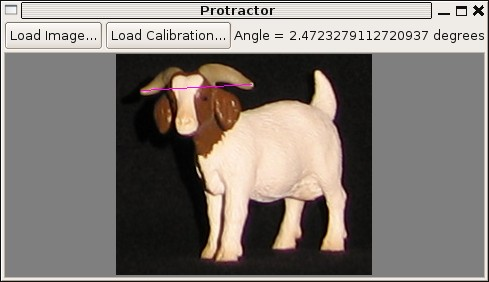
\includegraphics[width=0.7\textwidth]{screenshots/protractor_goat}
 \caption{The protractor tool.}
 \label{fig:goat_angle}
\end{figure}

The protractor tool converts a camera into a $3D$ version of the $2D$ protractor you will have inevitably used to measure angles on a flat piece of paper.
This is not an analogy; the centre of the camera takes on the role of the protractors centre, so you will be measuring the angles through the centre of the camera, whilst the image captured by the camera takes on the role of the (usually) semi-circular part of a protractor where the degrees are marked.
One way of thinking about this is in terms of measuring the angles between rays of light that intercepted at the camera when it took a particular photo.

Unlike the physical protractor with its cumbersome interface we may here let the computer do the boring stuff, such as taking differences; the interface therefore consists of selecting two points in an image (It draws a line between them, the third side of the triangle as such.) - it then gives you the angle between these points.
See figure \ref{fig:goat_angle} for an example of measuring the viewing angle between the horns of a toy goat.

The interface is markedly simple. You need an image and a camera calibration for the camera which captured the image, as an \emph{.icd} file. This will usually be generated with camera calibration using a $2D$ target, see section \ref{intrinsic_calib} for details. The two buttons at the top left will load these. Once loaded you may click on the image to obtain you angles in the top right corner. Left clicking will snap the closest end of the line to the cursor, whilst right clicking will alternate between snapping one end or the other of the line to the cursor. The premise of this interface is that two right clicks set the rough position you want whilst further left clicks may then refine it. You may drag when you left click.



\section{Fundamental Calibration}
Write me.



\section{Triangulator}
Write me.



\section{Capture}
Whilst this button exists in the Windows version it only works in the Linux version. This is because it uses a Linux only library, lib-gphoto2\footnote{Hopefully it will be ported to windows at some point, as this would be very convenient for all involved. I would do it myself, but I do not have the time.}. If your running Windows you obviously arn't a professional however\footnote{No, I'm not apologising if you disagree.} and are unlikely to have any actual use for this section anyway.

Write me.



\section{Rectification}
Write me.



\section{Stereopsis}
Write me.



\section{Disparity To Mesh}
Given a disparity map for a rectified image pair and the related \emph{.pcc} file this will generate a 3D model.

Write me.



\section{Disparity Masking}
Given a disparity map allows you to extract the mask and save it for editing in a normal image editing program. You can then re-load the mask. Useful for removing parts of a disparity map to clean up dodgy/unwanted areas.

Write more.



\section{Disparity Cleaner}
This processes disparity maps in a bid to make them more aesthetically pleasing.
It provides two tools.
The \emph{Remove Spikes} button attempts to find statistically deviant sections of the disparity map and terminates them.
The \emph{Smooth} button smooths the map, filling in gaps in the disparity map as it does so.
By setting the \emph{Source Sd} parameter of the smoothing algorithm to $0$ it becomes an infilling algorithm, which interpolates and fills in gaps in the disparity map without changing already know disparity values.

Write more.



\section{Disparity Comparator}
Compares disparity maps, one disparity map should be a ground truth whilst the other is calculated by the algorithm being tested.

Write more.



\section{Disparity To Needle Map}
Write me.



\section {Scale}
Write me.



\section{Crop}
Write me.



\section{Crop Rectified Pair}
Given a pair of rectified images this allows you to crop both and update the \emph{.pcc} file so as to maintain consistency.

Write more.



\section{Scale Rectified Pair}
Given a pair of rectified images this correctly scales them whilst updating the related \emph{.pcc} file.

Write more.



\section{Warp}
Given the left image and disparity map of a rectified image pair this allows you to generate the right image as described by the disparity map. You can also interpolate between, and outside of, the two.

Write more.



\section{Super Warp}
Not yet implimented.



\section{Distorter}
Not yet implimented.



\section{Undistortor}
Given a photo taken by a camera and the \emph{.icd} file of that camera this will remove radial distortion from the image.

Write more.



\section{Cameras to Pair}
Given two \emph{.cam} files this will create a \emph{.pcc} file to represent them as a stereo pair.

Write more.



\section{Pair to Cameras}
Given a \emph{.pcc} file this splits it into a \emph{.cam} file for each camera.

Write more.



\section{Swap Pair}
Swap around a pair file, such that the left camera becomes the right and vice-versa.

Write more.



\section{Camera Calibration}
Uses a 3D calibration target to calibrate a camera to produce a \emph{.cam} file.

Write more.



\section{Camera to Intrinsic}
Given a \emph{.cam} file this extract the intrinsic parameters alone, as a {.icd} file.

Write more.



\section{Mesh to Disparity}
Given a 3D model and a rectified camera pair this will render the disparity map that will generate the visible parts of the 3D model. For calculating a ground truth disparity map given a ground truth 3D model.

Write more.



\section{Mesh Wibbalizer}
Write me.



\section{Render Mesh}
Write me, after critical fixing bugs.



\section{Visualise}
Not yet implemented.



\section{Colour Matching}
A simple tool to match the colours of a stereo pair.

Write more.



\section{Homography}
Allows you to apply a homography to an image, most useful for extracting textures from planer surfaces in an image so they can be easily worked with/used else where.

Write more.



\section{Anaglyph}
Write me.



\section{Crop Disparity}
Write me.



\section{Scale Disparity}
Scales a disparity map, so you can do Stereopsis to produce a high resolution disparity map and then down-res it for visualisation.

Write more.





\section{File Info}
Provides a breakdown of the information within the three \emph{simple} file types used  by the program:
\begin{itemize}
\item \emph{.icd} file. Represents a cameras intrinsic calibration. That is its intrinsic matrix and radial distortion parameters, as well as the dimensions of the images to which is applies.

\item \emph{.cam} file. Represents both the intrinsic and extrinsic parameters of a single camera. Contains a projection matrix and radial distortion parameters, which get broken down into position and orientation etc by this tool for display.

\item \emph{.pcc} file. Represents two cameras, including there intrinsic and extrinsic parameters as well as the fundamental matrix for them.
\end{itemize}
Opening any one of the aforementioned files with this tool with the load button will produce textual information in regards to its contents. Obviously, this tool is only of value if you actually understand the information contained, or have another program which you can transfer it into.



\section{Capturing Advice}
\label{capture_advice}
This section gives advice on capturing input; this is entirely about how to take two photos that will work well with this tool.
Divided into four sub-sections it first covers the camera to use, then advice on taking the photo, followed by advice on the relationship to use between cameras. The final sub-section covers what kind of scenes work best.

\subsection{Choice of Camera}
This has already been touched on, and in truth unless you are a photographer you probably only have a single camera to choose from anyway, but for those who have a choice I shall endeavour to provide some gauge as to which choice is best.
I already stated that you get what you pay for, and this is roughly true, but see the below list, ordered from cheapest to most expensive.
\begin{itemize}
\item \emph{Mobile phone camera}. Forget it. Ok, you will get something if you follow my advice on image quality in the next section, in an ideal situation. But its just not worth the hassle for the crap that will come out the other side. Mobile phone cameras are at best a gimmick, they have no real world value other than to sell mobile phones.

\item \emph{Compact camera}. What most people have. These cover a large range of capabilities, some are terrible, some are reasonable, and there size is convenient enough that you can casually keep one on you most of the time. Most are sold at a mega-pixel resolution that is a lie however, they tend to be very noisy, and the automatic procedures of Cyclops are not very noise friendly. You will probably need to reduce noise, either by scaling the images or blurring, as covered in the next section.

\item \emph{Prosumer camera}. SLR shape, compact camera performance. Price tag in the middle. Yeah, you get a prosumer camera you are wasting your money. If you are willing to carry around a SLR shaped camera it might as well \emph{be} an SLR, even if the SLR is last years model. This is not strictly fair, some of them do a good job, but there mostly just statistics orgies, with all the lies that follow. The biggest issue is that they tend to still have small sensors, so they don't capture more light and hence get all the noise of the compacts. They regularly have lenses that are pushed far outside there optical capabilities, which cause problems with distortion that Cyclops has to compensate for. Because of this you might be better off using a compact than one of these.

\item \emph{SLR}. Size matters. When it comes to genitalia and cars this point can be argued, but when it comes to cameras it is a matter of basic physics. The larger the lens and sensor the more light you can capture. The more light the better the photo in every way. SLR's live this; you can take a photo with an SLR and throw it straight at Cyclops, no problems. The inter-changeable lenses are also invaluable. There are a whole load of other reasons why they are better than anything else (Speed...), but there not as relevant to cyclops.
\end{itemize}
If you have to choose between cameras in the same category its all about light capture - go for the largest sensor and the largest lens. Of course, the first rule of photography always applies - the only camera that matters is the one you have when you want to take a photo; but one tends to plan to use Cyclops rather than use it on a whim.
If you have an SLR and a choice of lenses then its all about accuracy of calibration, a prime lens is best because its calibration is as close to constant as is reasonably obtainable.
Otherwise its the consideration that you will be using the fully zoomed out or fully zoomed in position that counts, so choose a good lens that matches the scene as best you can.


\subsection{Image Quality}
This can be divided into two parts, actually taking the photos and then post-processing the photos before giving them to Cyclops.
This entire section comes down to one principal, that Cyclops does not appreciate artistic beauty, it is a set of algorithms that like photos to be as sharp as possible. This only applies to the automatic approach, for the manual approach all that matters is that you can use the photos. That often means a lot of the same things though, so worth keeping in mind even for the manual approach.

\subsubsection{Shooting}
Most of the usual rules of photography apply, but there is some variation:
\begin{itemize}
\item Every photographer knows this, but to re-iterate: Bright scenes will be sharper, as the shutter can fire quicker, if there is not enough light use a tripod and/or flash (But see below.). A sharp scene makes stereopsis much easier, and is better for making 3D models anyway as you want good sharp textures.

\item Whilst it will work if you use the flash its prefable not to, for the fully automatic approach. It doesn't matter if your manually placing points in the triangulator. As the scene is static consider a tripod and long exposure time instead. The problem with the flash is it matches the images presuming identical lighting; using a flash breaks that assumption. Because the camera, and hence flash, will not move that far between shots however you can often get away with it, as long as the scene is well textured. Of course, if you have an external flash not mounted on the camera then no problem exists.

\item Keep the camera still to avoid blurring, especially in low light. The exception is if the blurring is from motion blur, aligned with the epipolar lines - this does not matter as much, though its still best avoided. A good example of this situation is shooting from a moving car, if you aim out a window (See below.) and hold the camera still relative to the car and shoot two photos in rapid succession to create a stereo pair the direction of the blur will be along the epipolar lines, and consequently considerably less of a problem than otherwise.

\item Don't shoot through a dirty transparent surface. Cyclops will see the dirt and match it, this is not what you want. Even a surface that looks clean can cause problems, so best avoided altogether. Rain is also a bitch, though you can get away with rain as long as the drops are small enough to appear as noise rather than drops.

\item Avoid depth of field effects. It looks good to us humans, but Cyclops hates it. That means a high f-stop is desirable, which of course requires more light than a low f-stop to avoid a slow shot. You can additionally improve accuracy by using the same aperture for all calibration shots and then all shots using the resulting calibration, as calibration will change with the f-stop.

\item When choosing your scene consider its content. Large flat surfaces without texture will not work well, whilst highly textured areas with intricate and unique detail are best. This makes old things ideal, as all that detail from being worn down with time makes the stereopsis algorithms life easier. Large flat areas with little detail will usually be presumed planar, this is fine if they actually are, but not so good if they are not. This makes modern curvy buildings regularly problematic.
\end{itemize}

\subsubsection{Post-processing}
Given a noisy image, which you will get from most non-SLRs except when outside on a sunny day, it is best to remove the noise, even at the expense of image sharpness.
A blurry image with low noise is better than a sharp image with lots of noise.
There are two ways to do this, either reduce the image resolution or use an image editor with a blurring function.
Blurring is preferred, though reducing image resolution can be easier and just as effective as you can get the camera to do it or do it within Cyclops as a matter of course when preparing the rectified image pair.
If blurring then a Gaussian blur, maybe with edge preserving, is preferred.
The level of size reduction/blurring should be manually set to get rid of most of the noise.

A further issue that is critically important for the stereopsis step is that the two images should be colour matched. If your unfortunate enough to take a stereo pair where the cameras white balance changes between the two photos then it will need correcting. Cyclops provides a tool to do this, the \emph{Colour Matching} tool.


\subsection{Camera layout}
Excluding a single failure point Cyclops can be made to work with photos taken of the same object in any relative positions.
But some positions work far better than others.
The rule of thumb is to match the layout of our eyes - two photos taken side by side without rotation. (But see below for discussion on the gap size.)
\begin{itemize}
\item The distance between the two cameras is the hardest to get right, its ultimately down to experience. The closer two cameras are to each other the easier it is to match pixels together and the more reliable the output will be. But the closer together the two photos the more an error matters, and the further apart they are the more accurate triangulation will be. Its simply a matter of finding the sweet spot for the scene in front of you - this is all relative to how far away the scene is and how large the scene is. A larger scene will require a larger gap to get a good resolution on the depth calculation. To give some clue the tutorial scene was shot with a gap that is about 30 times smaller than the distance to the scene. That is probably a smaller than optimal gap however, maybe 15 or 10 times smaller would of been better.

\item Rotation is best avoided. The automatic fundamental calibration can only cope with a very limited amount before it fails and you have to do it manually. The rest of the system is far more robust to rotation, so you can take a fair bit if you are willing to do the fundamental calibration manually. But more rotation (as does a larger gap) leads to more occlusion, areas of the scene that can not match in the other photo because they are not there. These are best minimised.

\item Being able to see the position where the other photo was taken in either image of a stereo pair is fatal. Being able to almost see it is also usually fatal, and at the very least going to create unreliable results. Avoid doing this at all costs. The reason is two fold. At the projection of one camera in another\footnote{By this I mean that if two people were to take a stereo pair with two cameras simultaneously then if either photo includes the other camera then where you see that camera in the photo is this point.} triangulation can not work, its degenerate, and as you get close to this point the slightest error has an astronomical consequence, so this is bad for both the automatic and manual approach. Rectification in the automatic approach has to make the image larger and larger as the projection of the other camera gets closer to being visible. When the projection of the other camera is visible the image size is infinite. Avoiding this is quite easy - just don't move forward or backwards when moving from the first photo to the other, and make sure any such motion is greatly exceeded by horizontal/vertical translation.
\end{itemize}


\subsection{Scenes}
You can in principal shoot anything, as long as it does not move between the two photos.
Unless you have a special rig that means static scenes only really.
What counts as movement depends on how much there is between photos, so it matters more for objects closer to the cameras.
Cooperative adults are quite doable, though children and pets are often not, unless tranquilised.
Architecture and landscapes (On a windless day.) make the best subjects.
For one thing, they complain less when they come out all distorted.
There are some practicalities however:
\begin{itemize}
\item Shininess (Specularities) are a major problem - don't expect anything shiny to work well. The problem is in the stereopsis step, where as the camera moves so do the specularities, yet they get matched regardless of the fact they have moved creating lumps in the output. Stereopsis on a car usually produces something closer to a sea urchin. Eyeballs cause hell, especially as getting them to stay still between photos is a nightmare. This is also another reason to keep the gap small, as a larger gap makes this problem worse. The further away a specular object the less the specularities move however, so distant objects with specularities are not a problem.
\item Transparency. Does not work. With luck it will match whatever is on the other side of the glass etc, but it will also consider matching anything on the glass, such as dirt and logos. This can make a mess, especially if the transparent surface is also shinny. Again, being far away. or more importantly the areas being small and/or well divided up, much like windows in a building, will alleviate this problem.
\item Gratings, railings and the like. As previously mentioned, stereopsis is hard. Two images are not actually enough information alone to do it, we humans actually have two video streams, and can move our heads and eyes at will to gather more information, making it far easier for us. We also have a far poorer sense of depth than you might think - its fine at the precise spot we are looking, but in peripheral vision its not much good. Anyway, for Cyclops to work it has to make assumptions, and one of those assumptions is that changes of depth are rare. Put simply, it assumes the scene is mostly made up of smoothly changing surfaces with the occasional jump. Grates and railings break this assumption, and will generally fail to work. Normally, whatever is behind the railing will snap to the same depth as the railing itself, which can look very strange as you move around.
\end{itemize}
Reading the above you might think water to be the nemesis of this process. And in part you would be right, but its quite surprising how well it does on water considering how badly it should do. I'm not saying that a fountain would make a good subject though, that would fail, badly. But a river in your scene is not likely to be a total catastrophe.



\section{Technology}
Write me.



\section{File Formats}
Write me. (svt \& xml.)



\end{document}
